\documentclass[12pt]{article}
\usepackage[letterpaper, margin=1in]{geometry}
\usepackage{graphicx}
\usepackage{subcaption}
\graphicspath{{./images/}}
\usepackage{hyperref}
\usepackage{parskip}
\usepackage{amsmath}
\usepackage[framed, numbered]{matlab-prettifier}
\lstset{inputpath=../}
\usepackage{titlesec}

\titleformat*{\section}{\large\bfseries}
%\allowdisplaybreaks

\title{ELECENG 3CL4 Lab 3 Report}
\author{
    Aaron Pinto \\
    pintoa9 \\
    L02
    \and
    Raeed Hassan \\
    hassam41 \\
    L02
}

\begin{document}

\maketitle
\clearpage

\section*{Member Contributions} % copied from lab doc
Both group members contributed an even amount to both the exercises and the report. Both members went through the exercises together and contributed to all sections of the report.

\section*{Objective}
To design a proportional controller and a proportional controller with velocity feedback for the DC motor servomechanism, and explore trade-offs involved in the selection of the controller parameters and their impact on transient and steady-state responses of the control system.

\setcounter{section}{2}
\section{Experiment: Qualitative Trade-offs in Rise-time, Steady-State Error, Overshoot, and Settling Time for a Proportional Controller}
% talk about measurement procedure
In order to measure the peak overshoot (with respect to the final value) and steady state error, we measured the delta between the first peak and the steady state value using the peak finder tool for the peak and a cursor for the steady state value. The settling time measurement was performed by moving a cursor to the point at which the last oscillation was ending and the plot showed a straight line after. The time value shown on the cursor table was then taken as the settling time. The rise time was measured using a cursor as the time from 0 to the first instance of when the output reached the steady state value. We tried the "Bilevel Measurements" tool, but we found it to be inaccurate, though it did give us an approximation of where our values should be.

\begin{table}[h!]
\centering
\begin{tabular}{|c|c|c|c|c|c|c|} \hline
    $k_p$ & 0.5 & 1 & 2 & 3 & 4 & 5 \\ \hline
    peak overshoot (\%) & 0.7 & 38.4 & 54.7 & 65.7 & 75.3 & 82.4 \\ \hline
    steady-state error (deg) & 26.89 & 8.09 & 5.10 & 3.69 & 2.64 & 1.93 \\ \hline
    settling time (sec) & 0.336 & 0.469 & 0.618 & 0.771 & 0.881 & 1.067 \\ \hline
    rise time (sec) & 0.336 & 0.125 & 0.100 & 0.076 & 0.064 & 0.058 \\ \hline
\end{tabular}
\caption{\label{table:exp1_measurements}Measurements for Experiment 1}
\end{table}

% observations or something here
We measured values at a $k_p$ of 0.5, 1, 2, 3, 4, and 5. As we increased the gain, we observed that the peak overshoot percentage increased, the steady state error decreased the settling time increased, and the rise time decreased. This matches what we expected from our theoretical calculations in the pre-lab and from what we've observed in previous labs. % The settling time increases because the system is underdamped and as we increase $k_p$ the real part of the poles decrease (the poles approach the $j\omega$-axis), and the the constant $\tau_m$ is defined as $\frac{1}{Re(pole)}$ and for a moderately underdamped system, $T_s$ is $\approx 8\tau_m$.

\section{Experiment: Proportional Controller Design}
% calculations
To determine the values for $k_p$ that would meet the design specifications (produce underdamped with maximum overshoot of 50\%, 55\%, 60\%, and 65\%), we used the expression from the lab document to estimate the percent overshoot of an underdamped system. The expression was rearranged to solve for $k_p$ in Equation~\ref{eq:calc_kp}. The calculations to determine the values that would meet the specifications were done in MATLAB, with the MATLAB code shown in Listing~\ref{listing:exp2_calc_kp}. The values of $A$ and $\tau_m$ were the average of their determined values from time-domain and frequency-domain analysis in lab 2.
\begin{equation} \label{eq:calc_kp}
\begin{aligned}[b]
    P.O. &= 100\exp\left( -\frac{\pi}{\sqrt{4k_pA\tau_m-1}} \right) \\
    \ln\left(\frac{P.O.}{100}\right) &= -\frac{\pi}{\sqrt{4k_pA\tau_m-1}} \\
    \sqrt{4k_pA\tau_m-1} &= \frac{-\pi}{\ln\left(\frac{P.O.}{100}\right)} \\
    4k_pA\tau_m - 1 &= \left(\frac{-\pi}{\ln\left(\frac{P.O.}{100}\right)}\right)^2 \\
    4k_pA\tau_m &= \left(\frac{-\pi}{\ln\left(\frac{P.O.}{100}\right)}\right)^2 + 1 \\
    k_p &= \left( \left(\frac{-\pi}{\ln\left(\frac{P.O.}{100}\right)}\right)^2 + 1 \right) \ / \ 4A\tau_m
\end{aligned}
\end{equation}
\lstinputlisting[style=Matlab-editor, caption={Calculating $k_p$ to meet specifications}, label={listing:exp2_calc_kp}, lastline=6]{exp_calculations.m}

% measurement procedure goes here

\begin{table}[h!]
\centering
\begin{tabular}{|c|c|c|c|c|} \hline
    $k_p$ & 1.3314 & 1.7685 & 2.3395 & 3.3489 \\ \hline
    theoretical peak overshoot (\%) & 50 & 55 & 60 & 65 \\ \hline
    peak overshoot (\%) & 41.0 & 50.4 & 59.8 & 69.9 \\ \hline
    theoretical steady-state error (deg) & 7.51 & 5.65 & 4.17 & 2.99 \\ \hline
    steady-state error (deg) & 6.68 & 7.03 & 3.34 & 2.11 \\ \hline
    settling time (sec) & 0.53 & 0.51 & 0.58 & 0.70 \\ \hline 
\end{tabular}
\caption{\label{table:exp2_measurements}Measurements for Experiment 2}
\end{table}

%observations go here
Moving from our 1st to 2nd $k_p$, we observed some unusual behaviour where the steady state error increased and the settling time decreased, which is the opposite of what we expected to happen. We re-ran the test multiple times (in front of the TA as well) and still achieved the same results every time. Apart from this irregular result at a $k_p$ of 1.7685, the rest of the results followed the expected trend of peak overshoot increasing, steady state error decreasing and settling time increasing, as we increased our $k_p$.
\setcounter{section}{5}
\section{Joint Design of Proportional Controller and Velocity Feedback}
There are two design requirements to consider. We know that the magnitude of the steady-state error can be given by the expression $\left| e_{ss} \right| = \frac{\tau_d}{k_p}$. If the steady-state error at $k_p = 1$ is 10 degrees, to reduce the steady-state by a factor of 5 (to 2 degrees), we need to increase $k_p$ by a factor of 5. Therefore the design requirement for the magnitude of the steady-state error can be met by any $k_p > 5$. 
\begin{equation}
    \zeta = -\frac{\ln\left(\frac{P.O.}{100}\right)}{\sqrt{\pi^2 + \ln^2\left(\frac{P.O.}{100}\right)}}
\end{equation}
rearrange expression for $\zeta$ and $k_v$
\begin{equation}
\begin{aligned}[b]
    \zeta &= \frac{1+k_vA}{2\sqrt{k_pA\tau_m}} \\
    k_v &= \frac{2\zeta\sqrt{k_pA\tau_m}-1}{A} 
\end{aligned}
\end{equation}

\lstinputlisting[style=Matlab-editor, caption={Calculating $k_v$ to meet specifications}, label={listing:exp3_calc_kv}, firstline=8, firstnumber=8]{exp_calculations.m}

\clearpage
\appendix
\section{Experiment 1 Figures} \label{sec:exp1fig}
\begin{figure}[h]
    \centering
    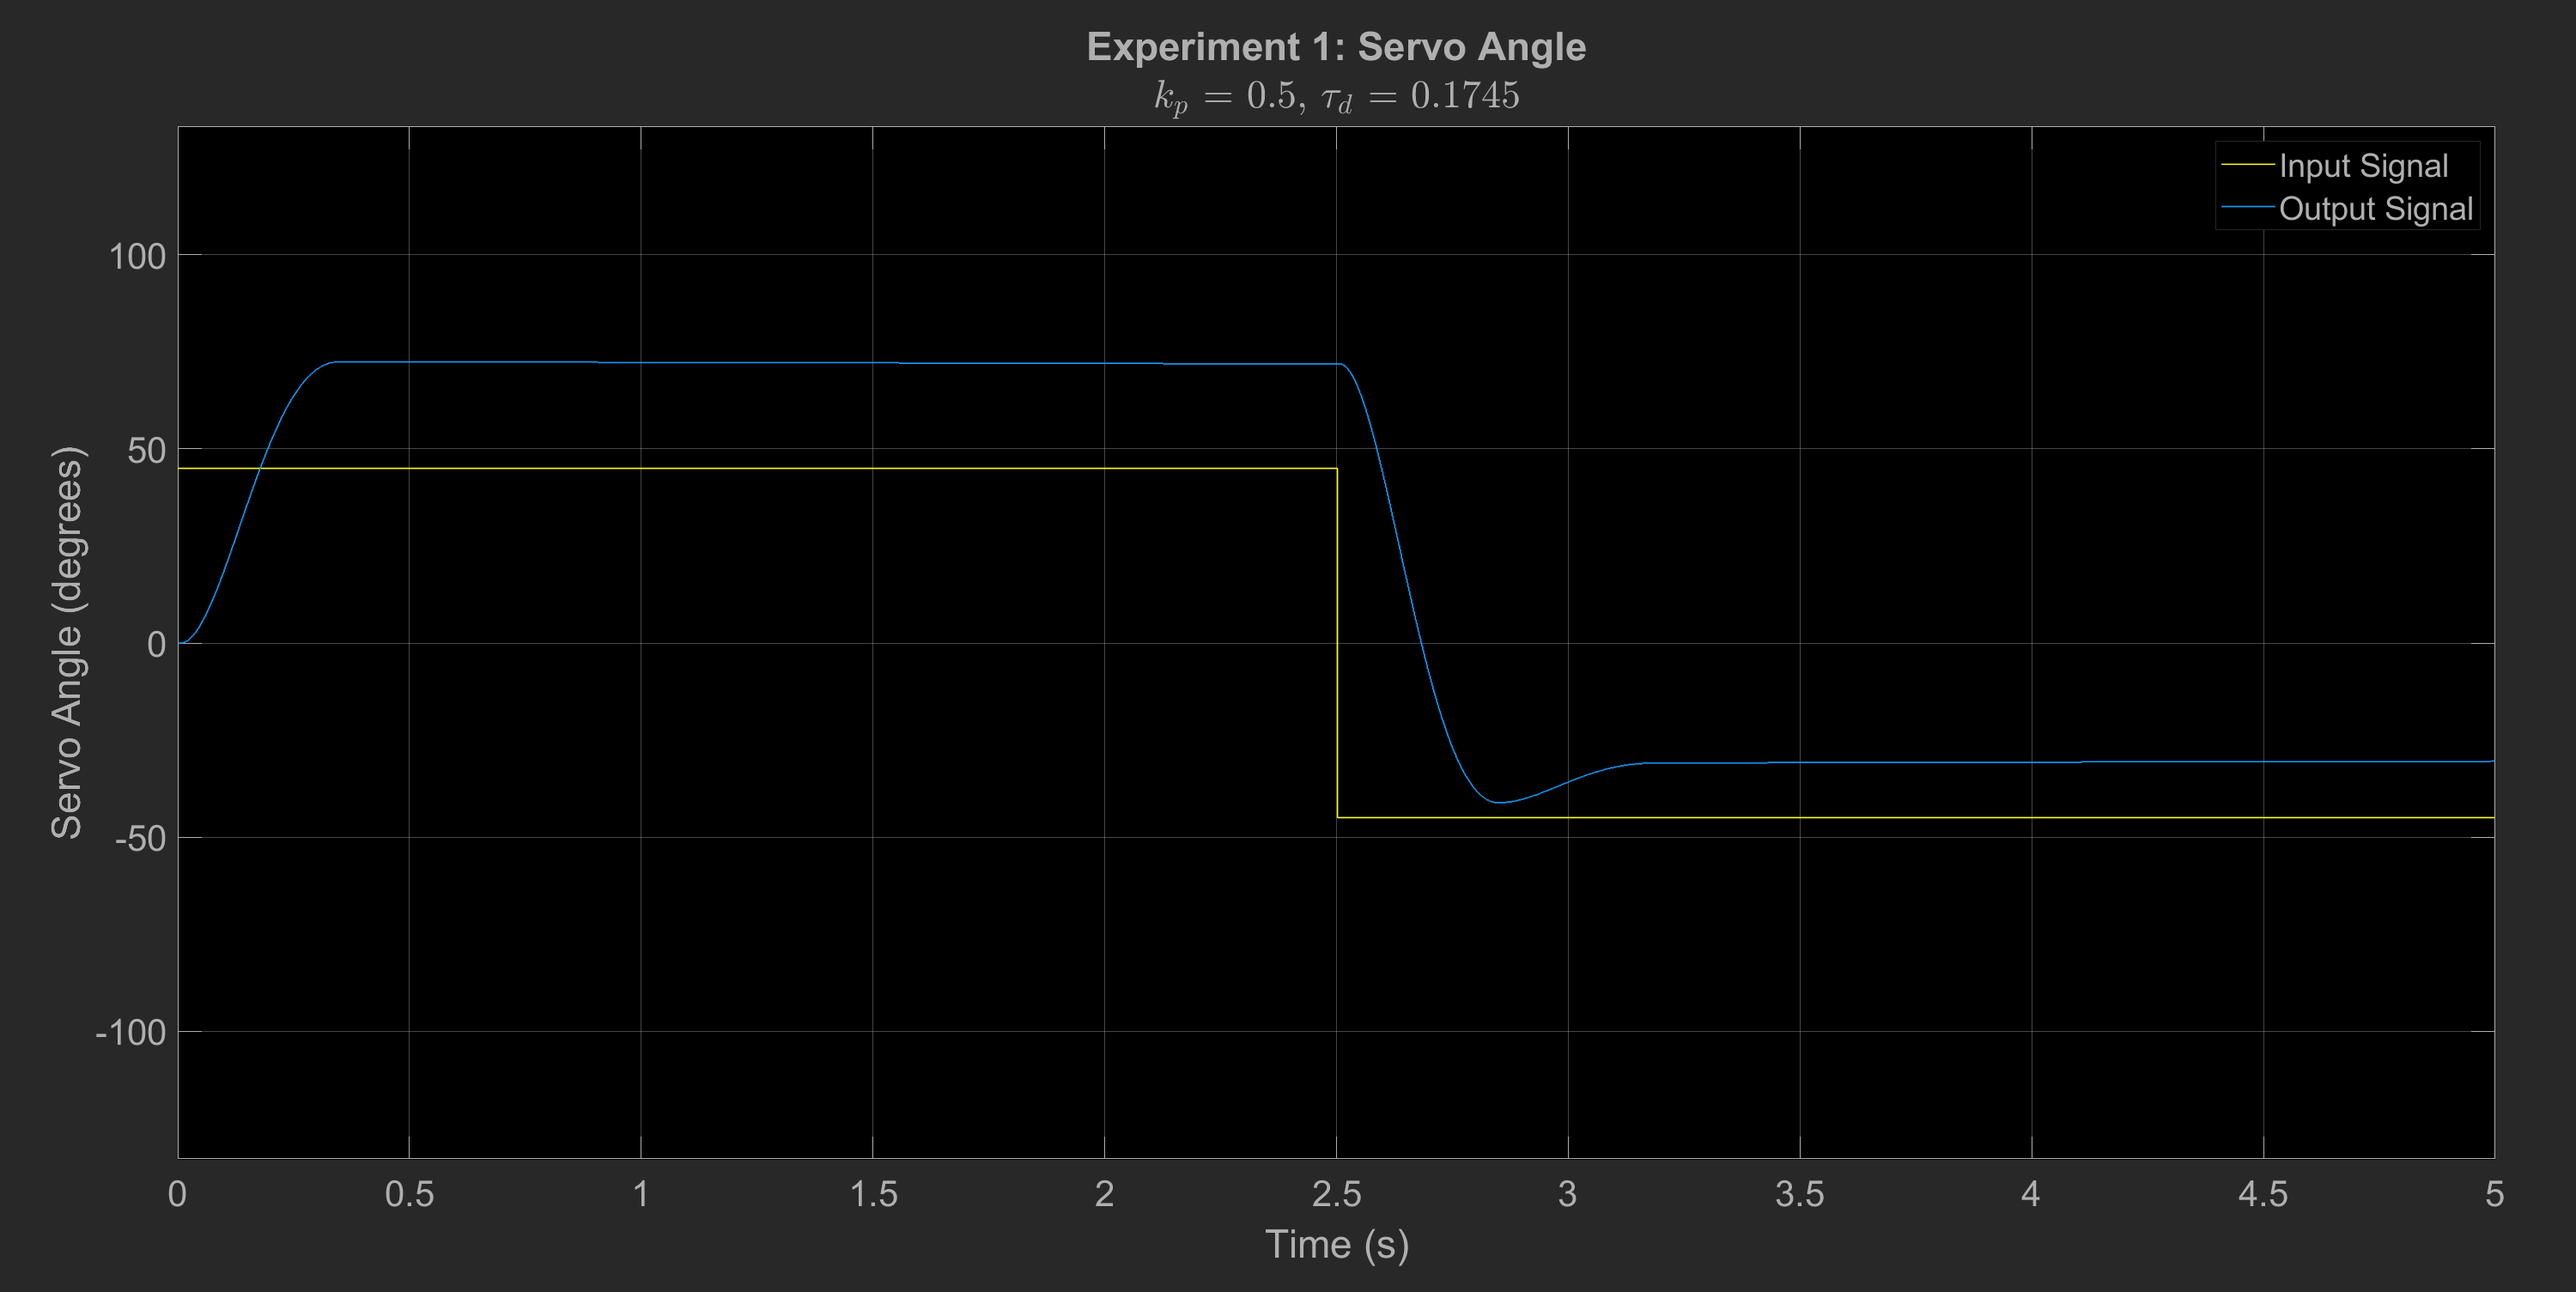
\includegraphics[width=0.91\textwidth]{exp1_kp0.5}
    \caption{Experiment 1: $k_p = 0.5$}
\end{figure}
\begin{figure}[h]
    \centering
    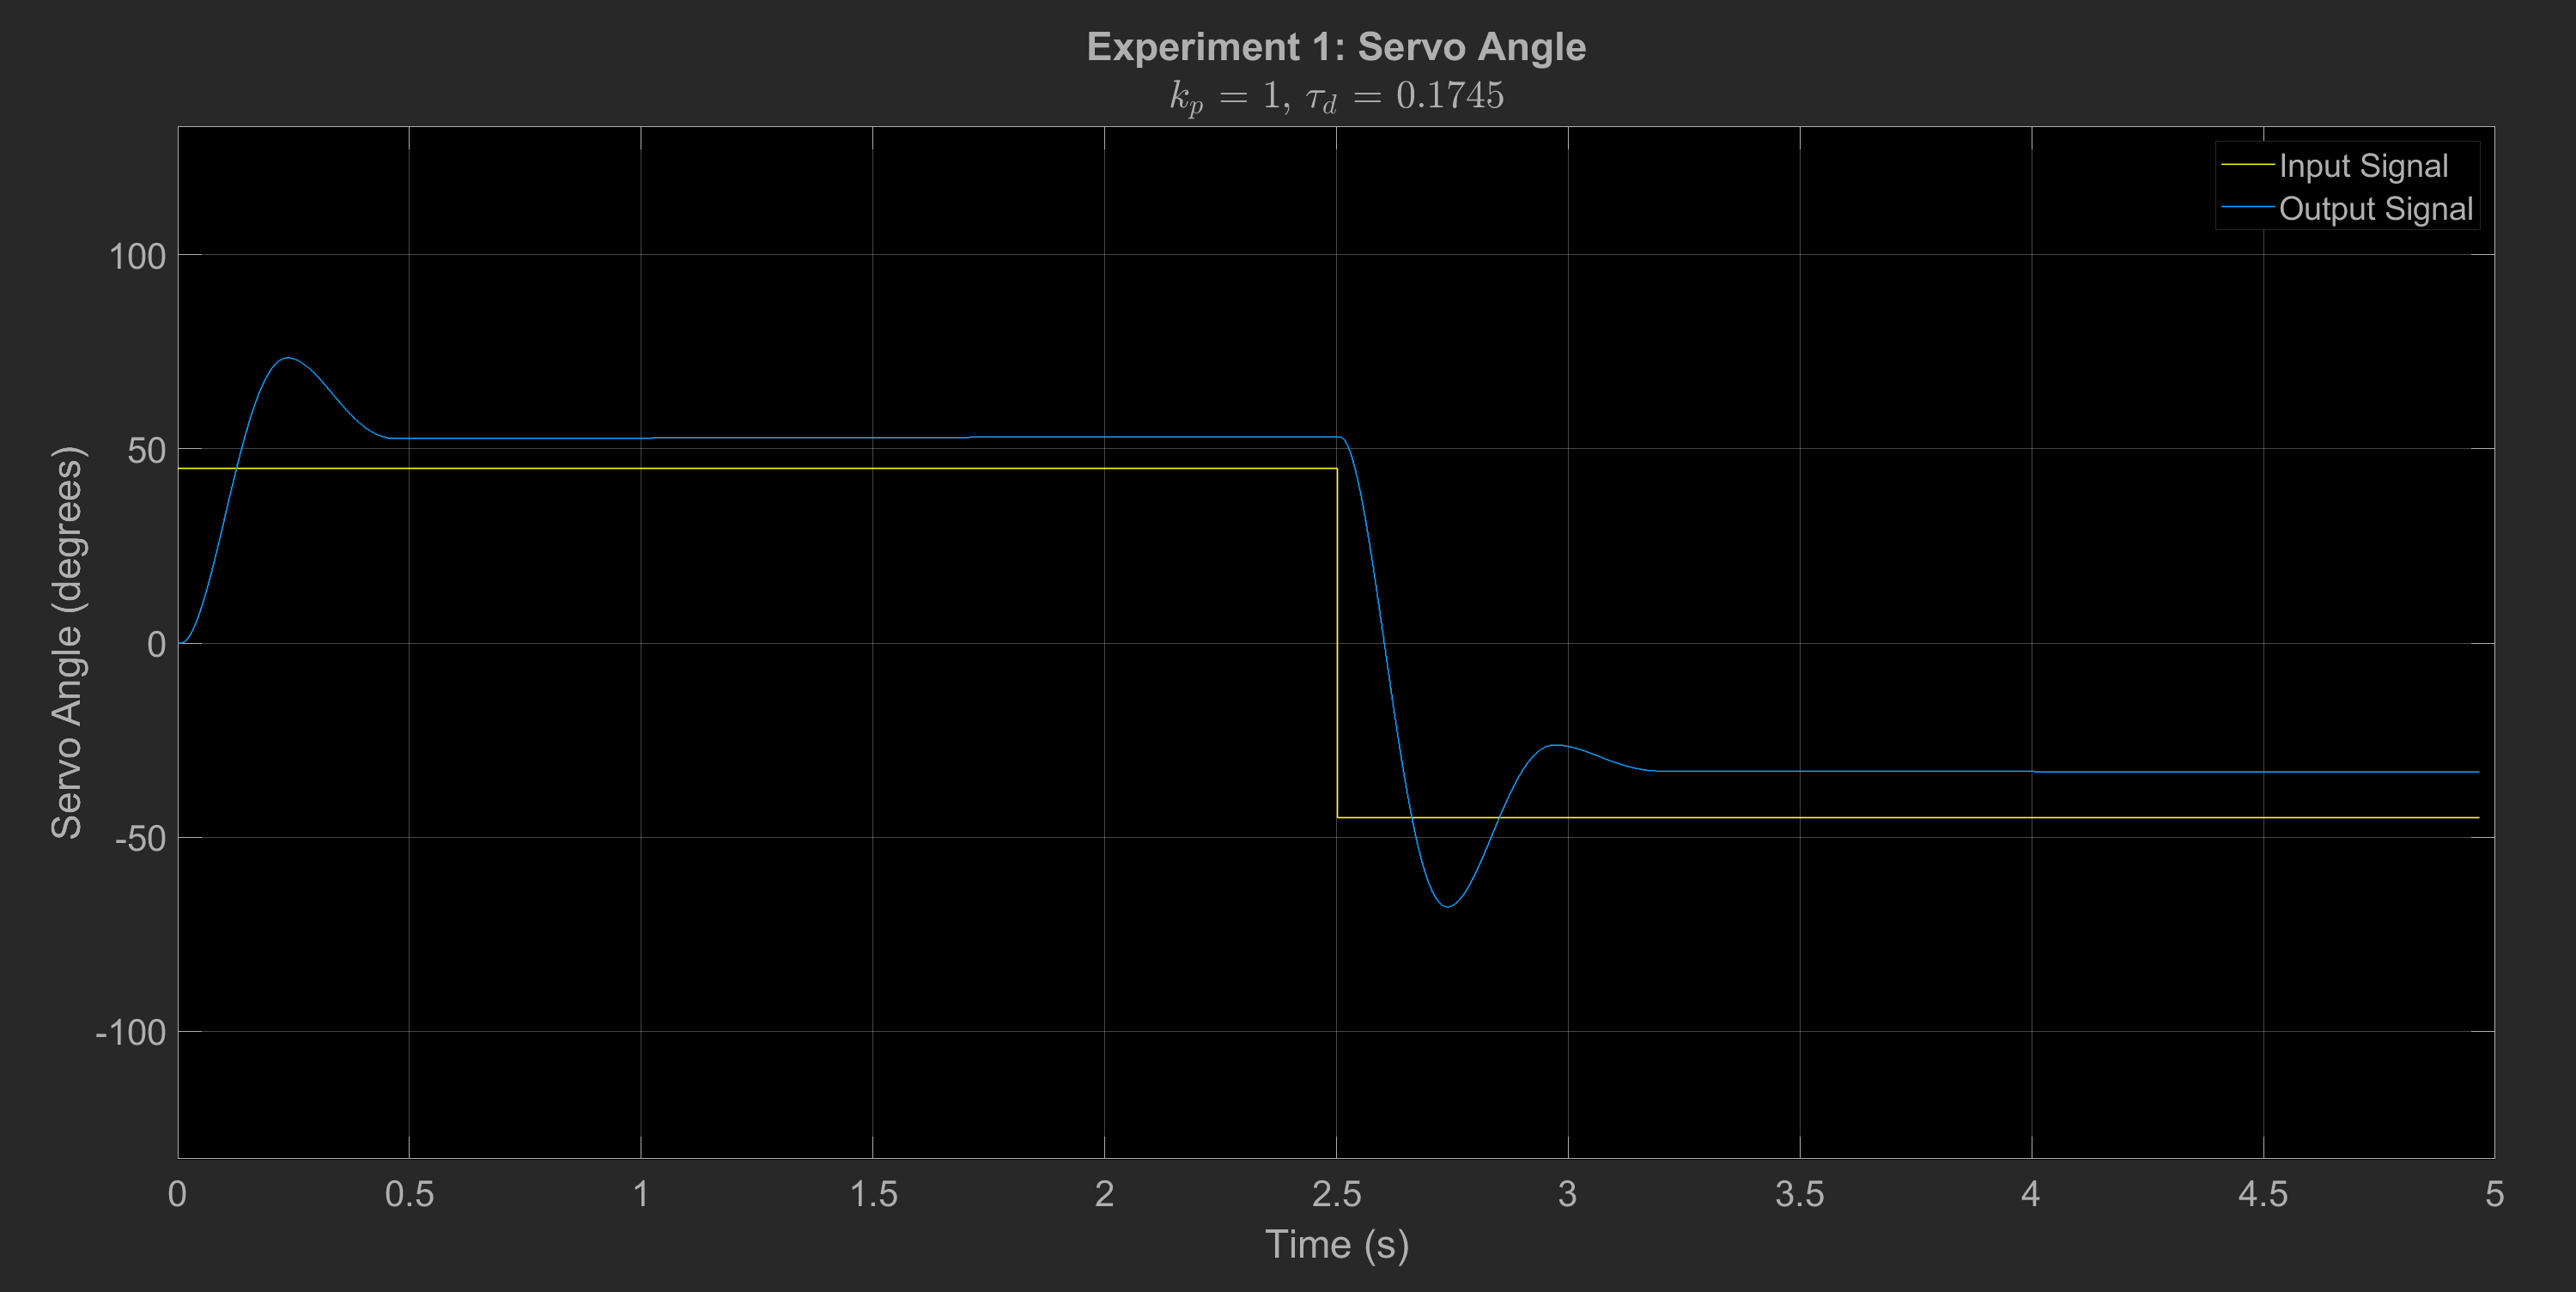
\includegraphics[width=0.91\textwidth]{exp1_kp1}
    \caption{Experiment 1: $k_p = 1$}
\end{figure}
\begin{figure}[h]
    \centering
    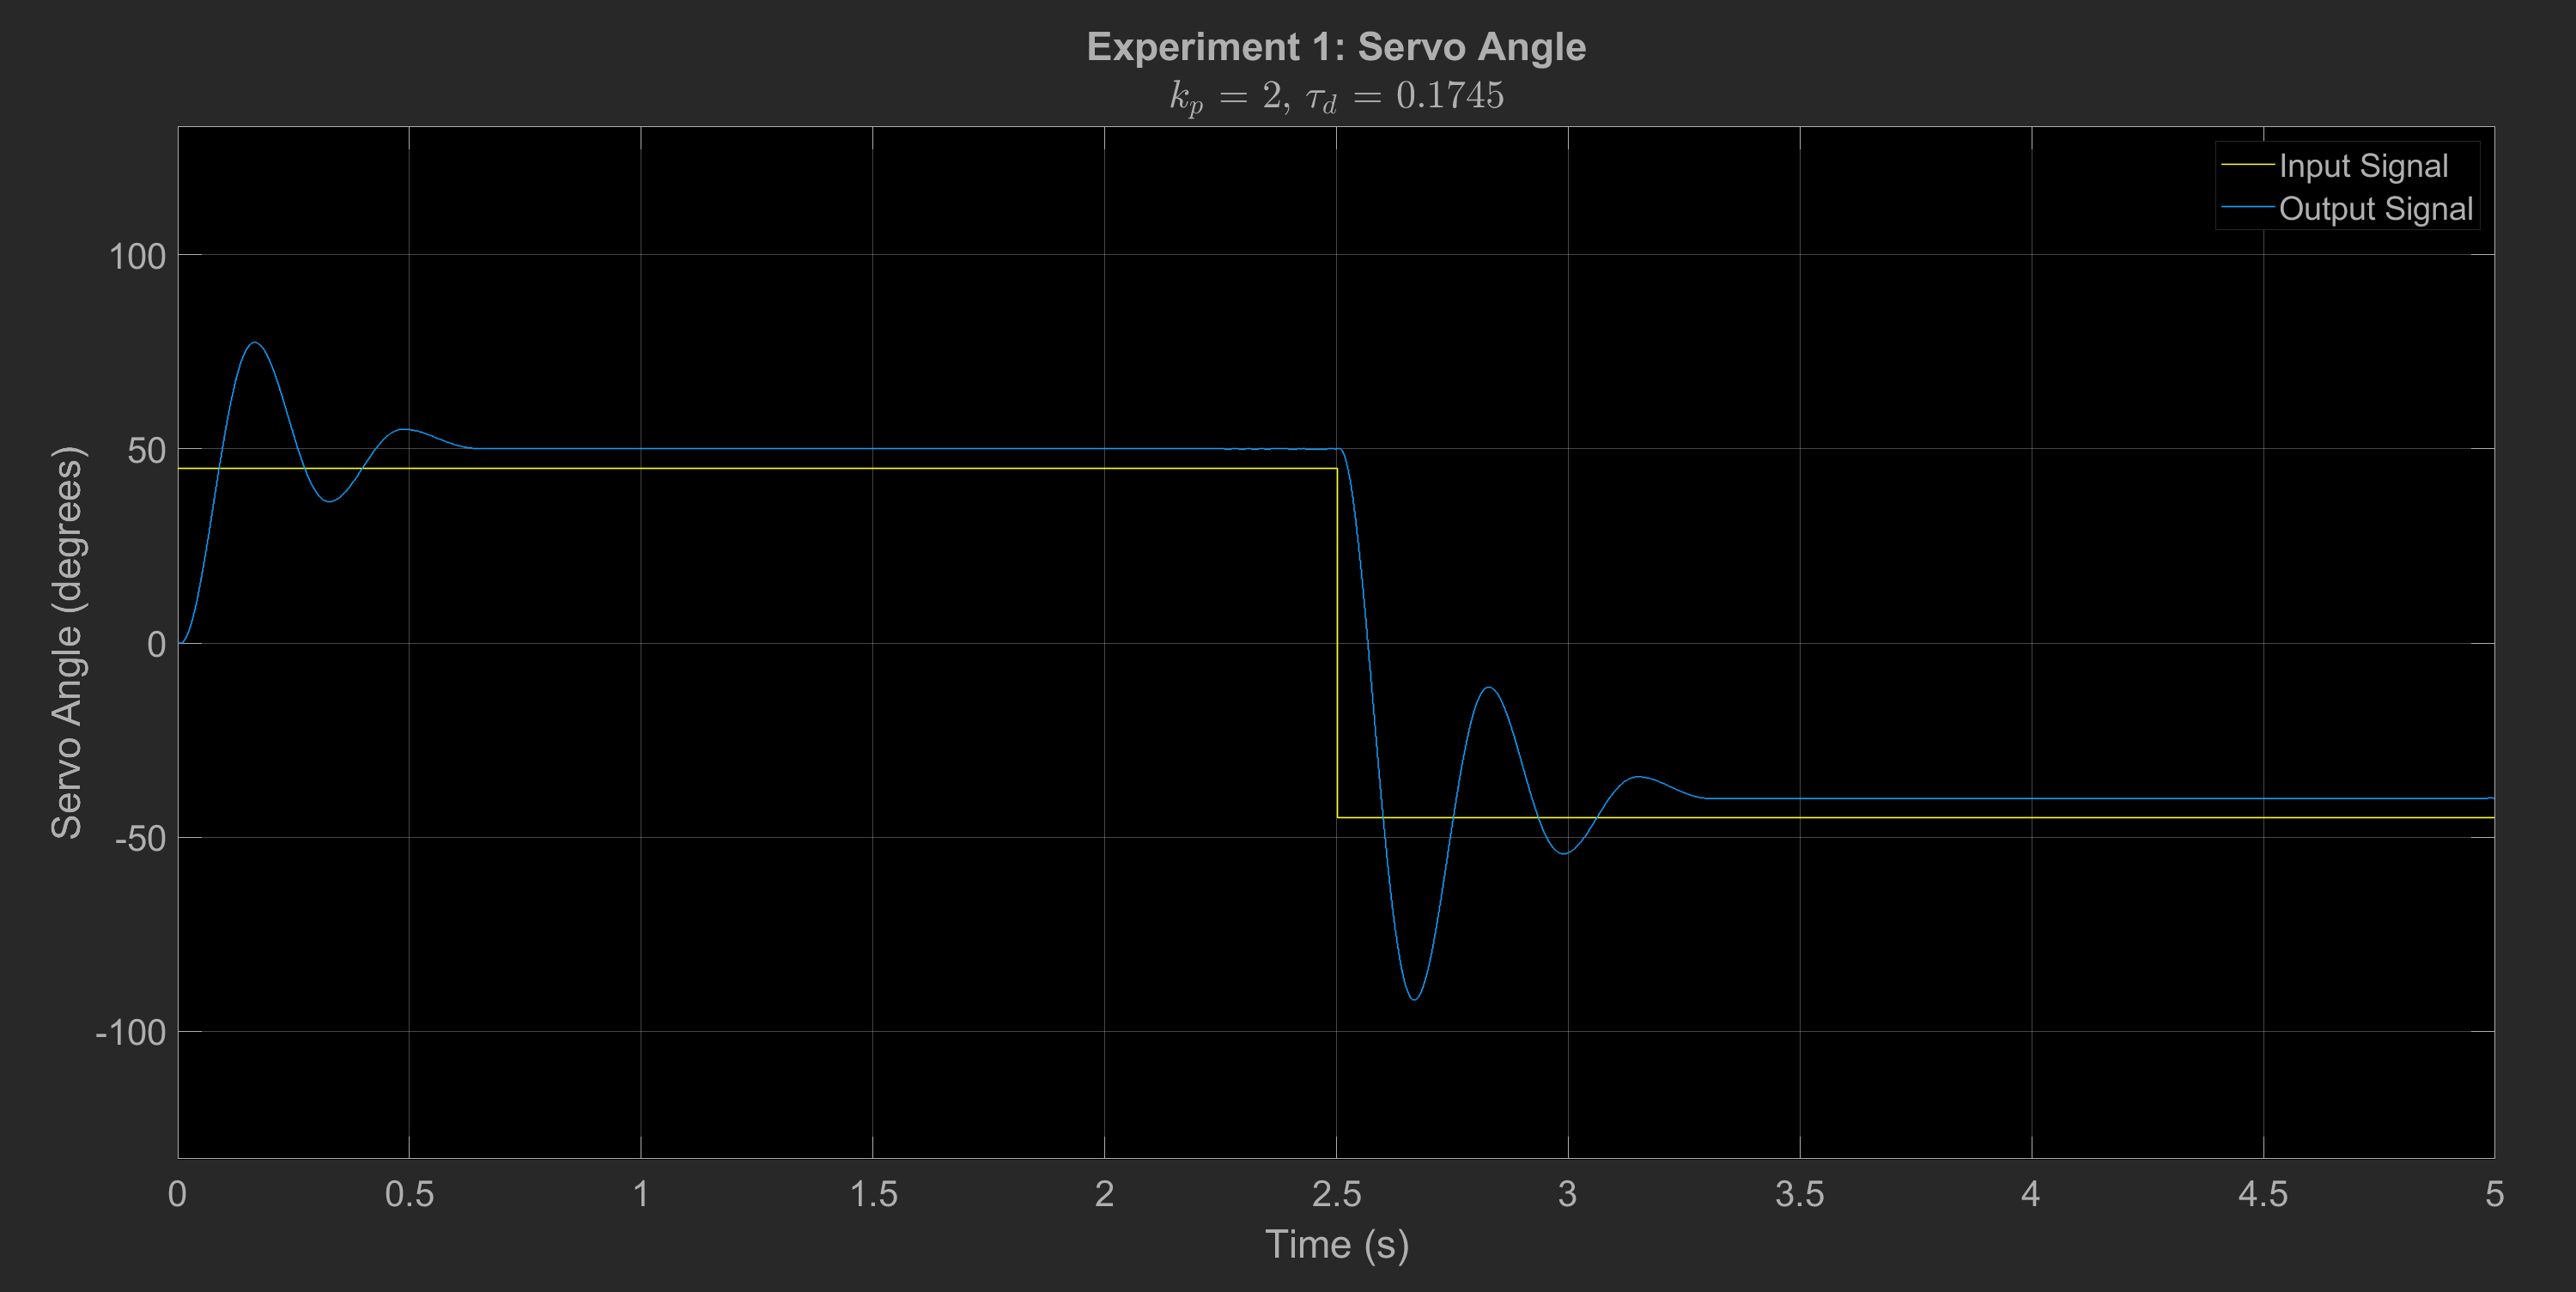
\includegraphics[width=0.91\textwidth]{exp1_kp2}
    \caption{Experiment 1: $k_p = 2$}
\end{figure}
\begin{figure}[h]
    \centering
    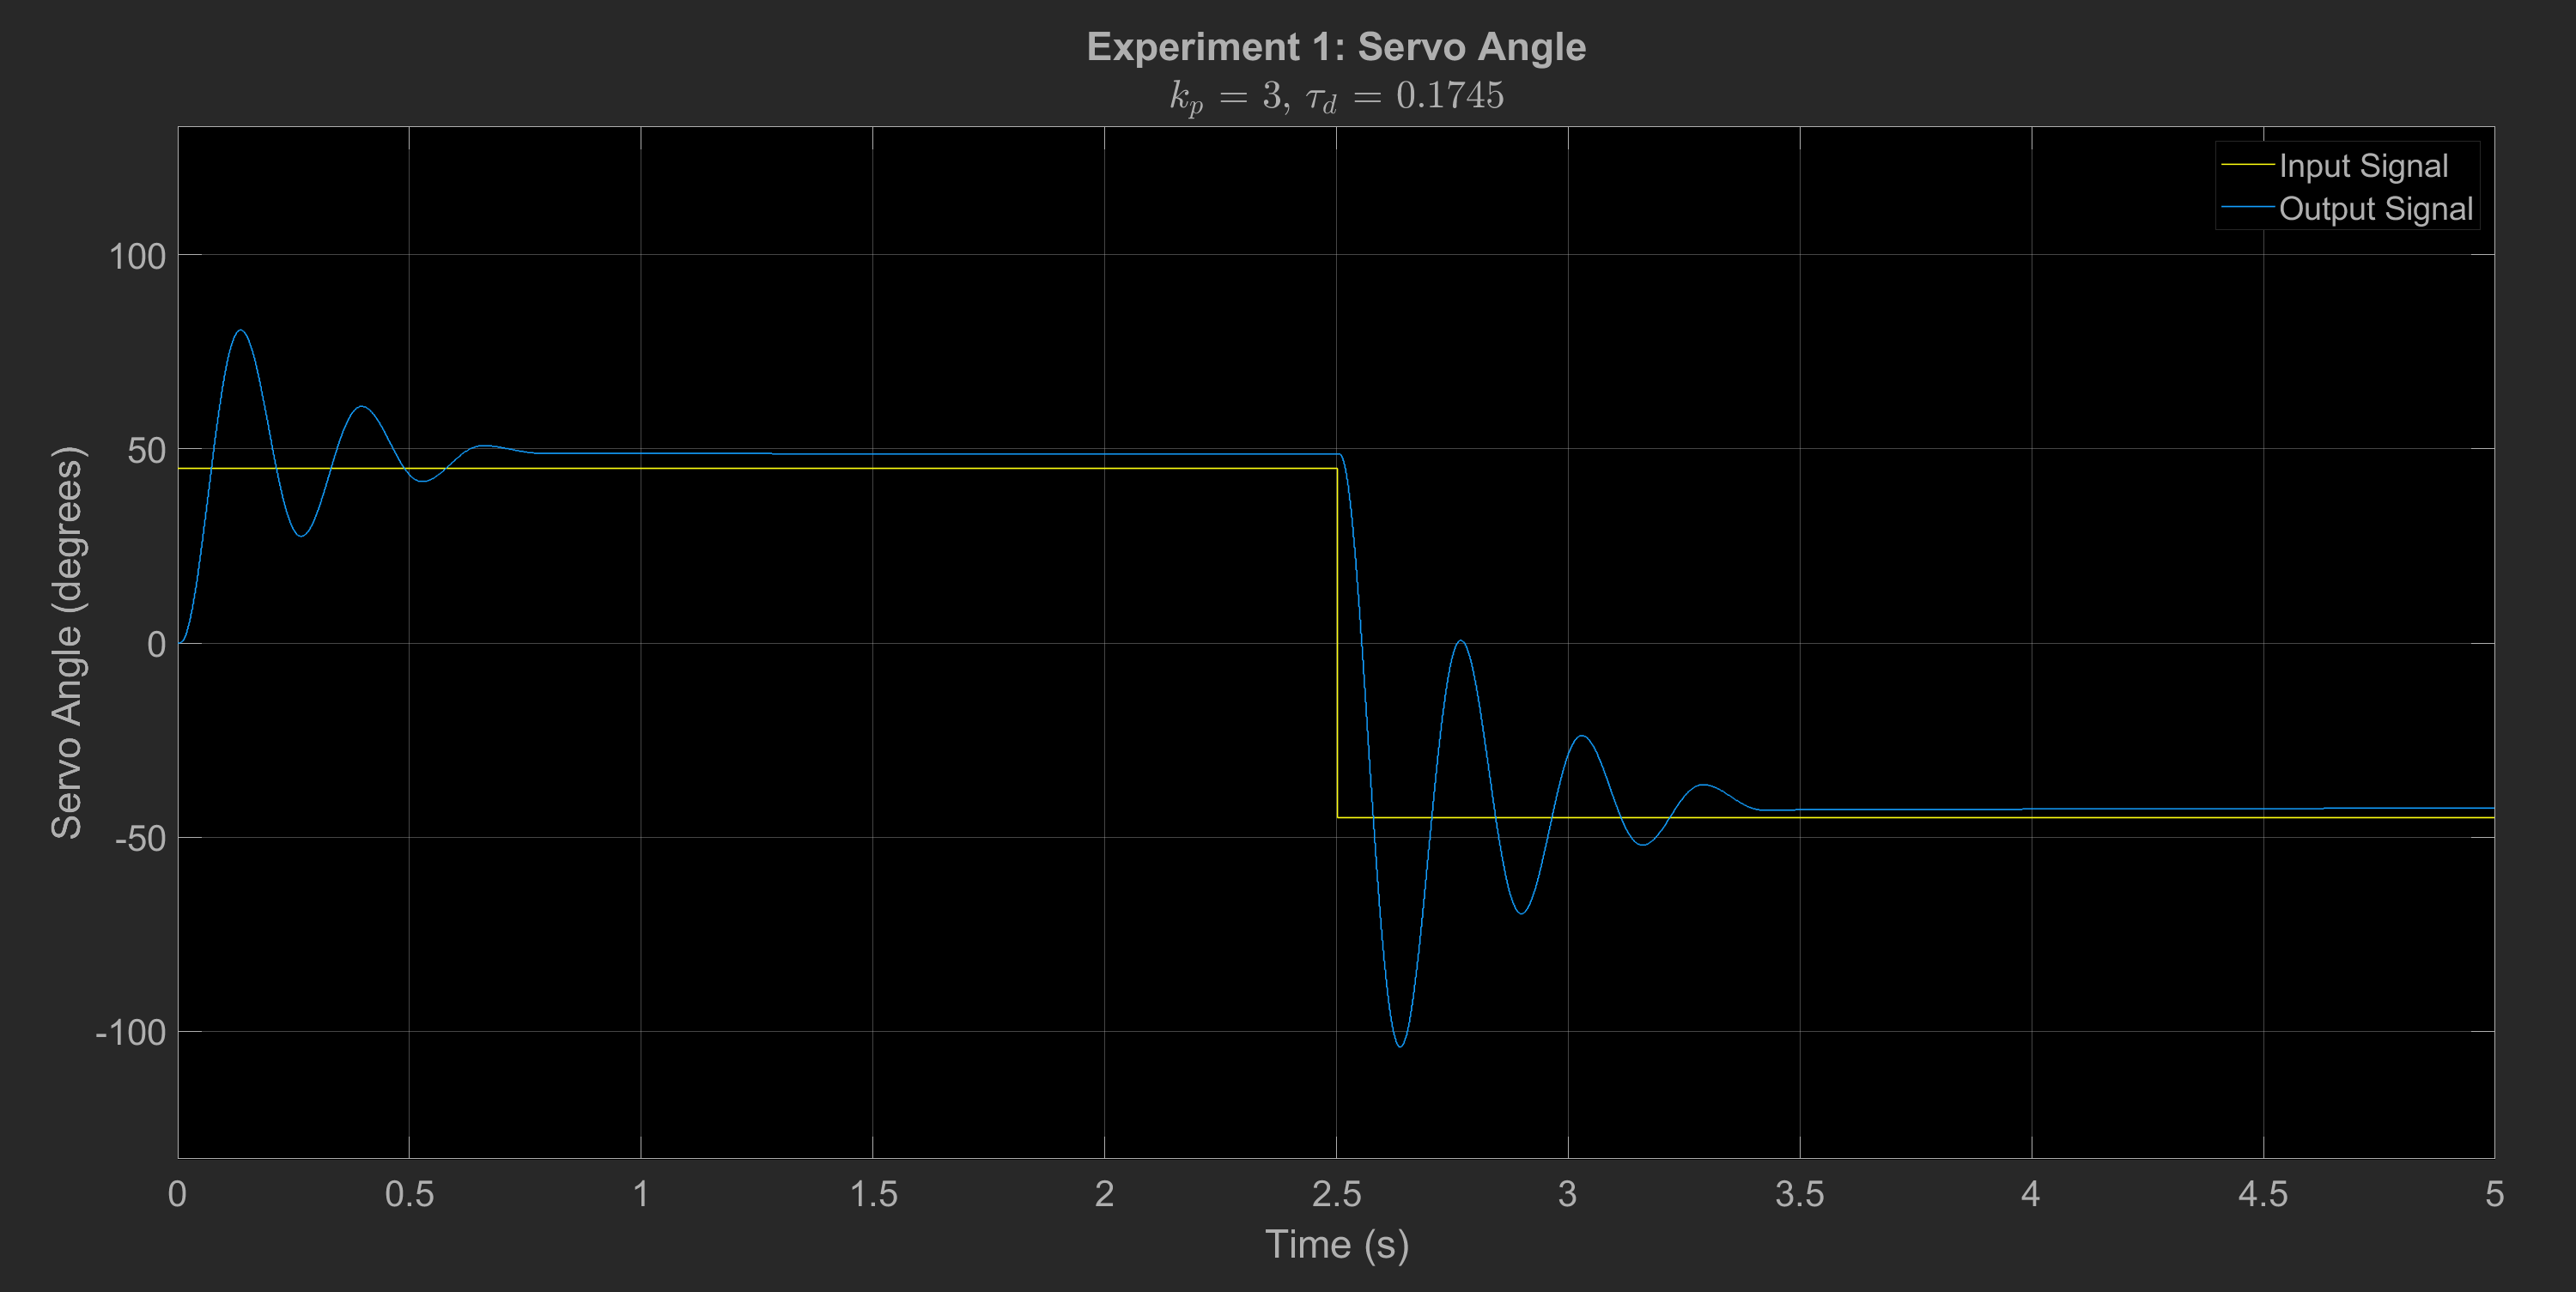
\includegraphics[width=0.91\textwidth]{exp1_kp3}
    \caption{Experiment 1: $k_p = 3$}
\end{figure}
\begin{figure}[h]
    \centering
    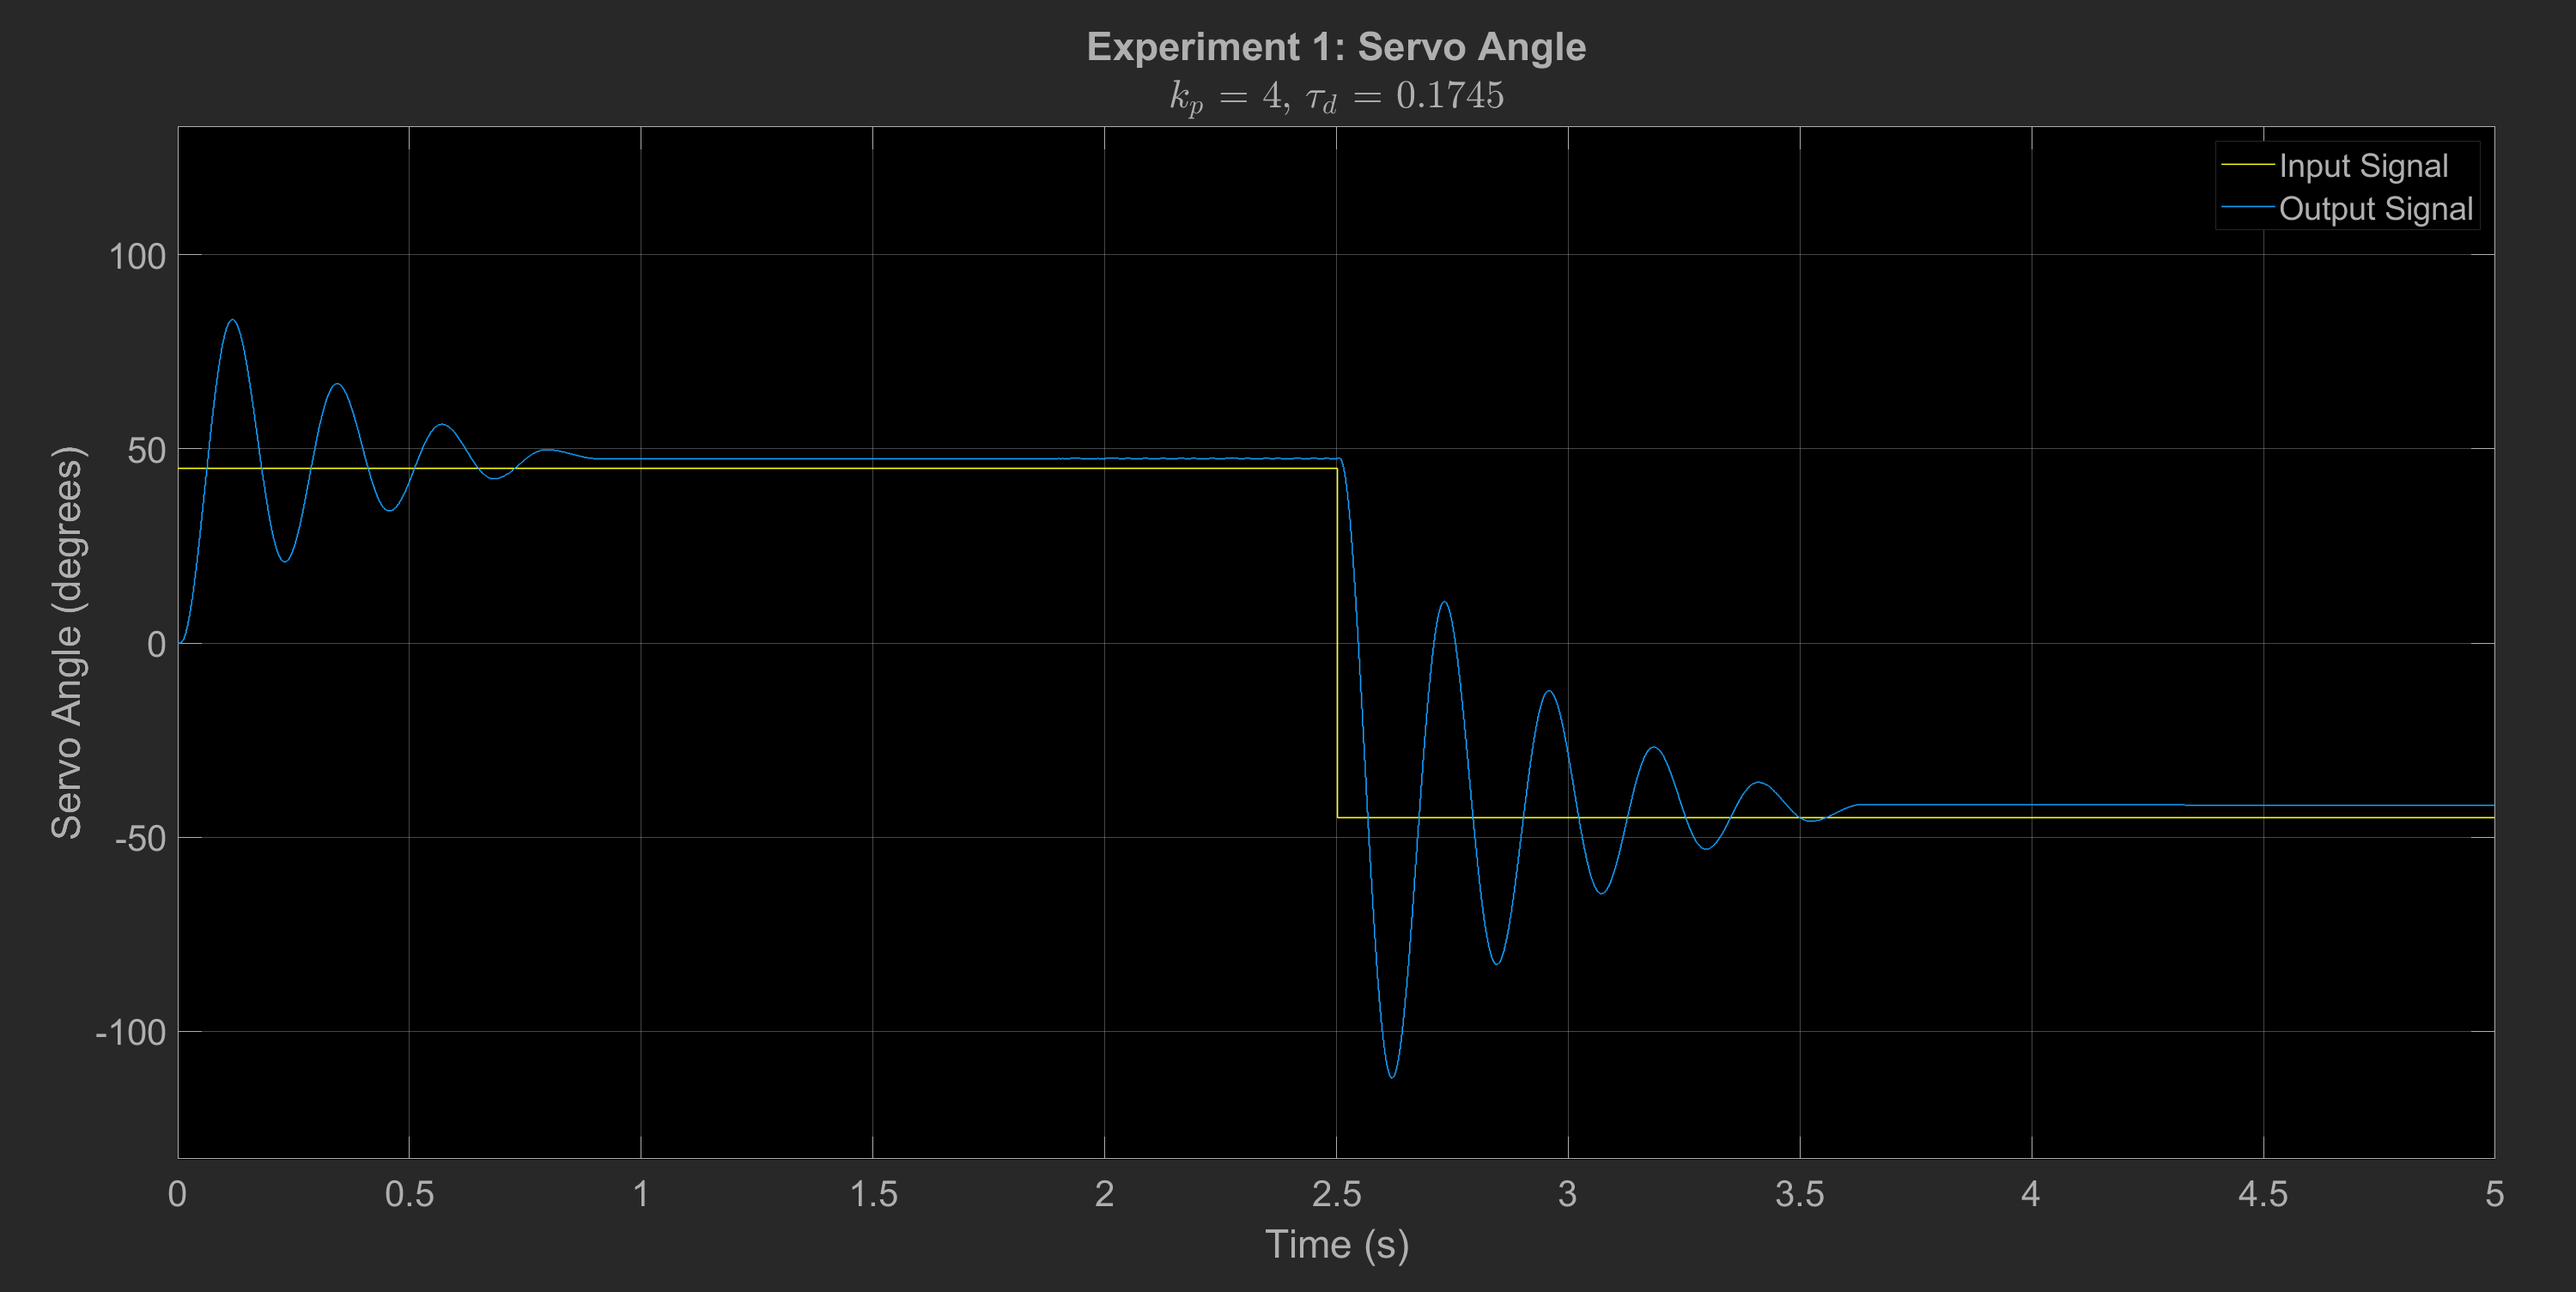
\includegraphics[width=0.91\textwidth]{exp1_kp4}
    \caption{Experiment 1: $k_p = 4$}
\end{figure}
\begin{figure}[h]
    \centering
    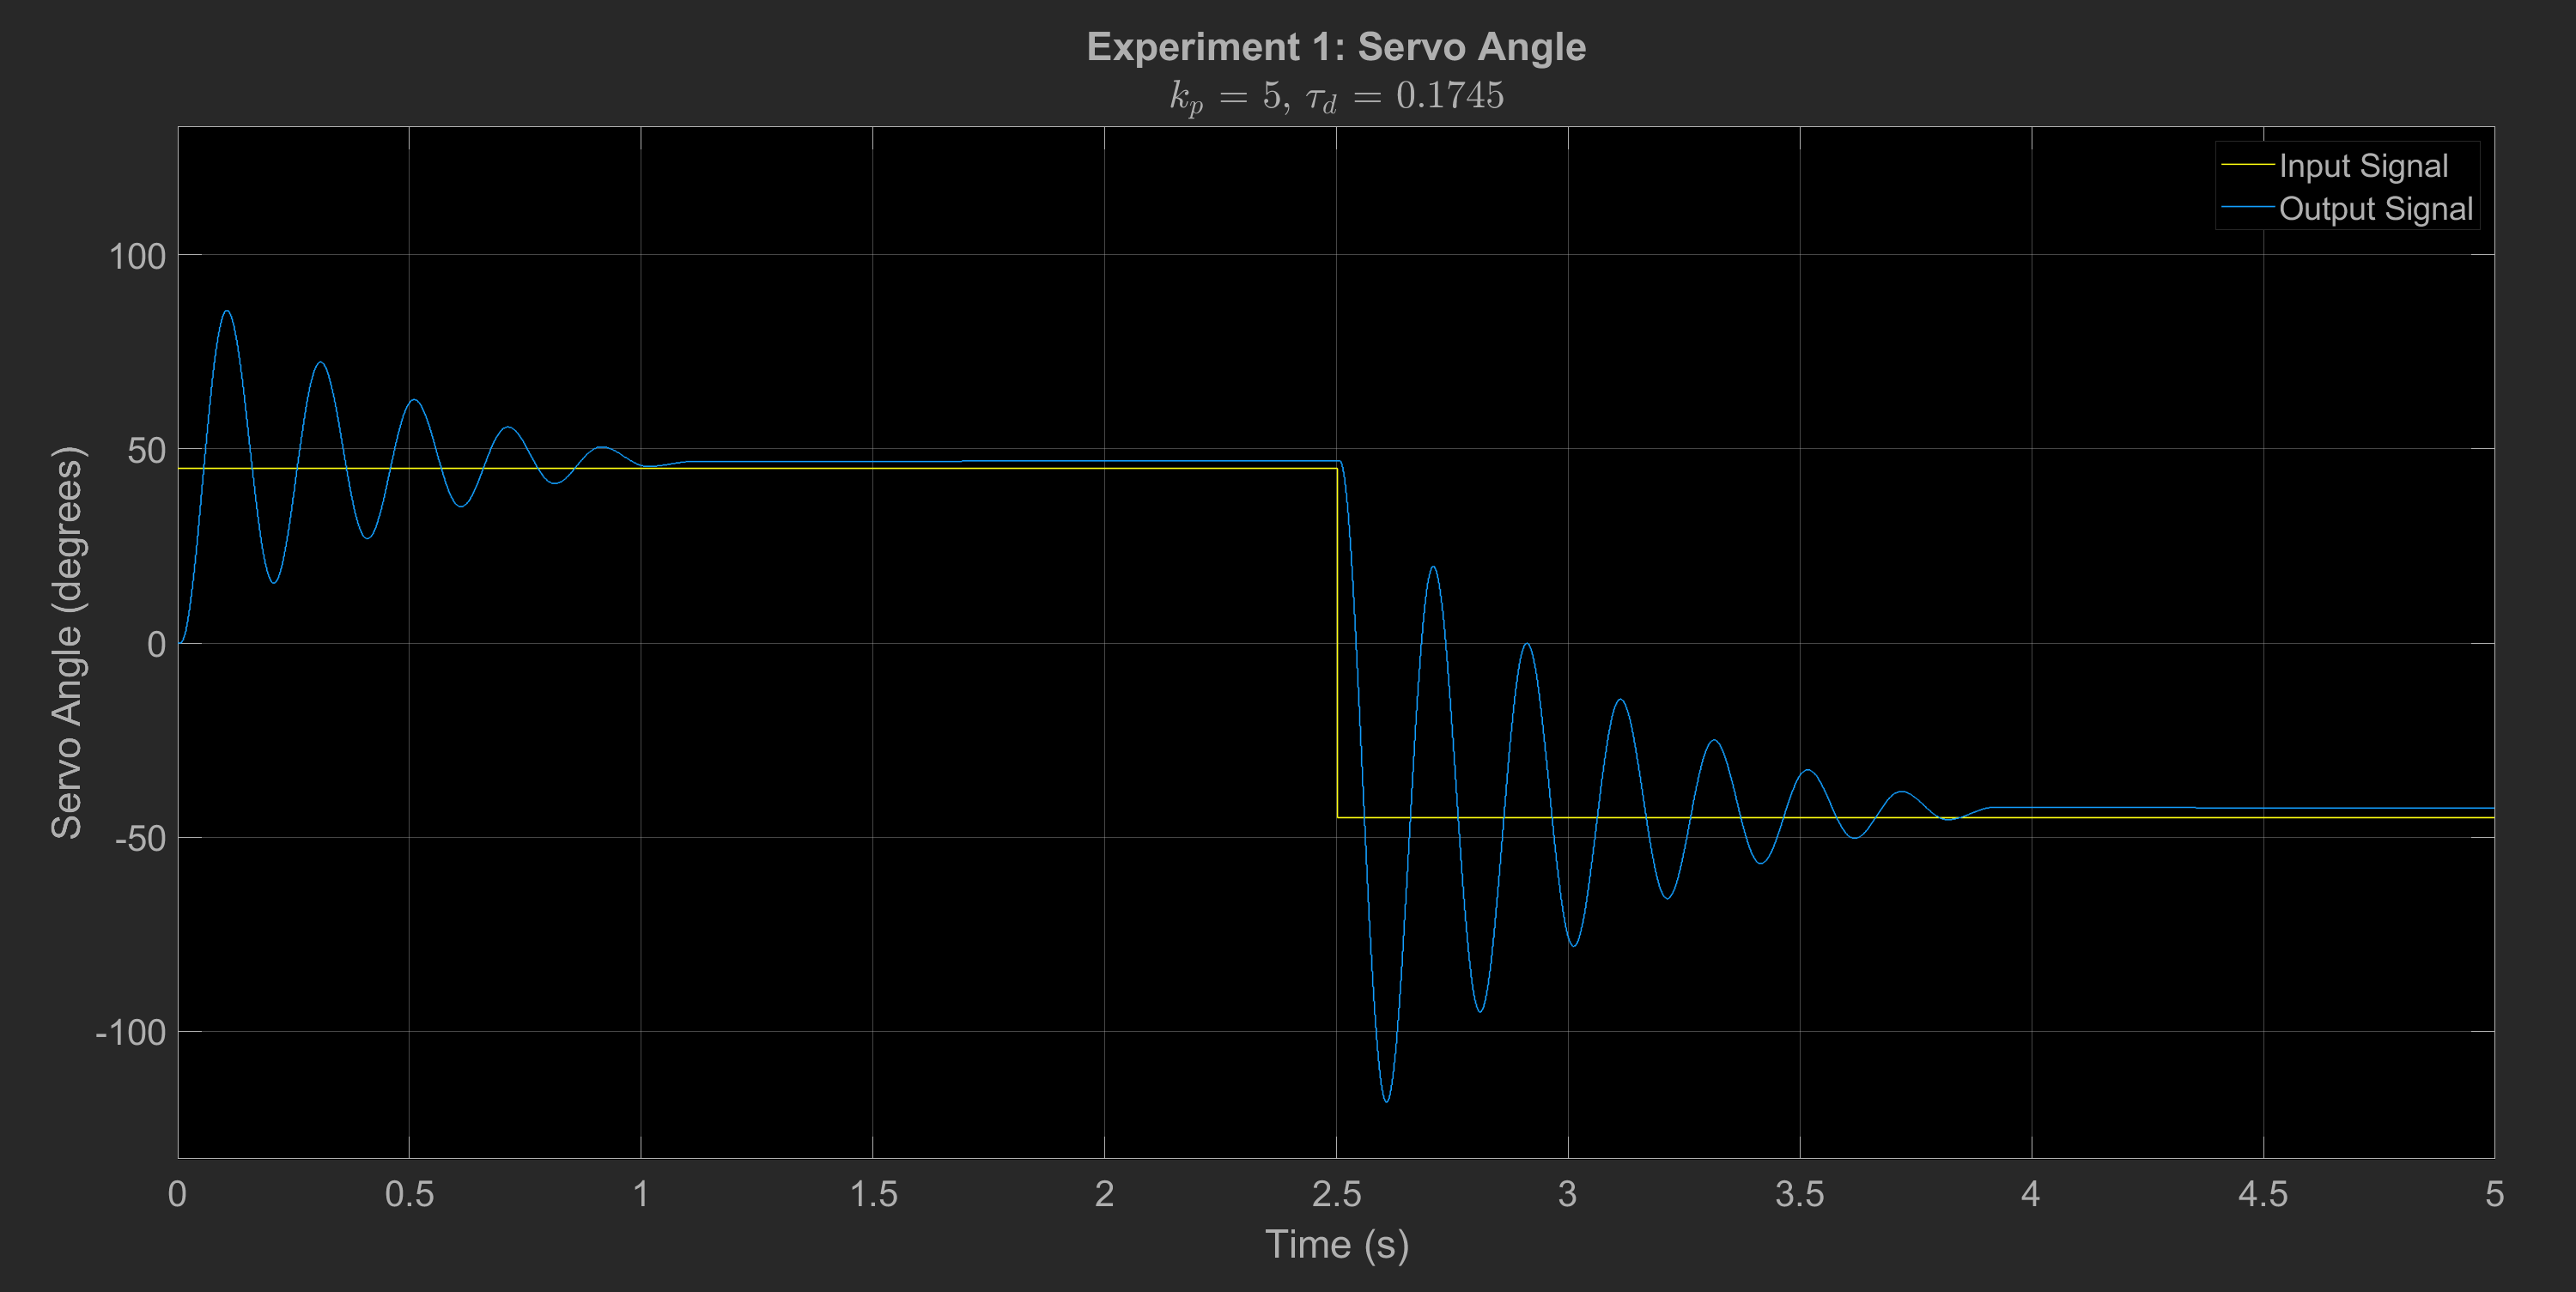
\includegraphics[width=0.91\textwidth]{exp1_kp5}
    \caption{Experiment 1: $k_p = 5$}
\end{figure}

\clearpage
\section{Experiment 2 Figures} \label{sec:exp2fig}
\begin{figure}[h]
    \centering
    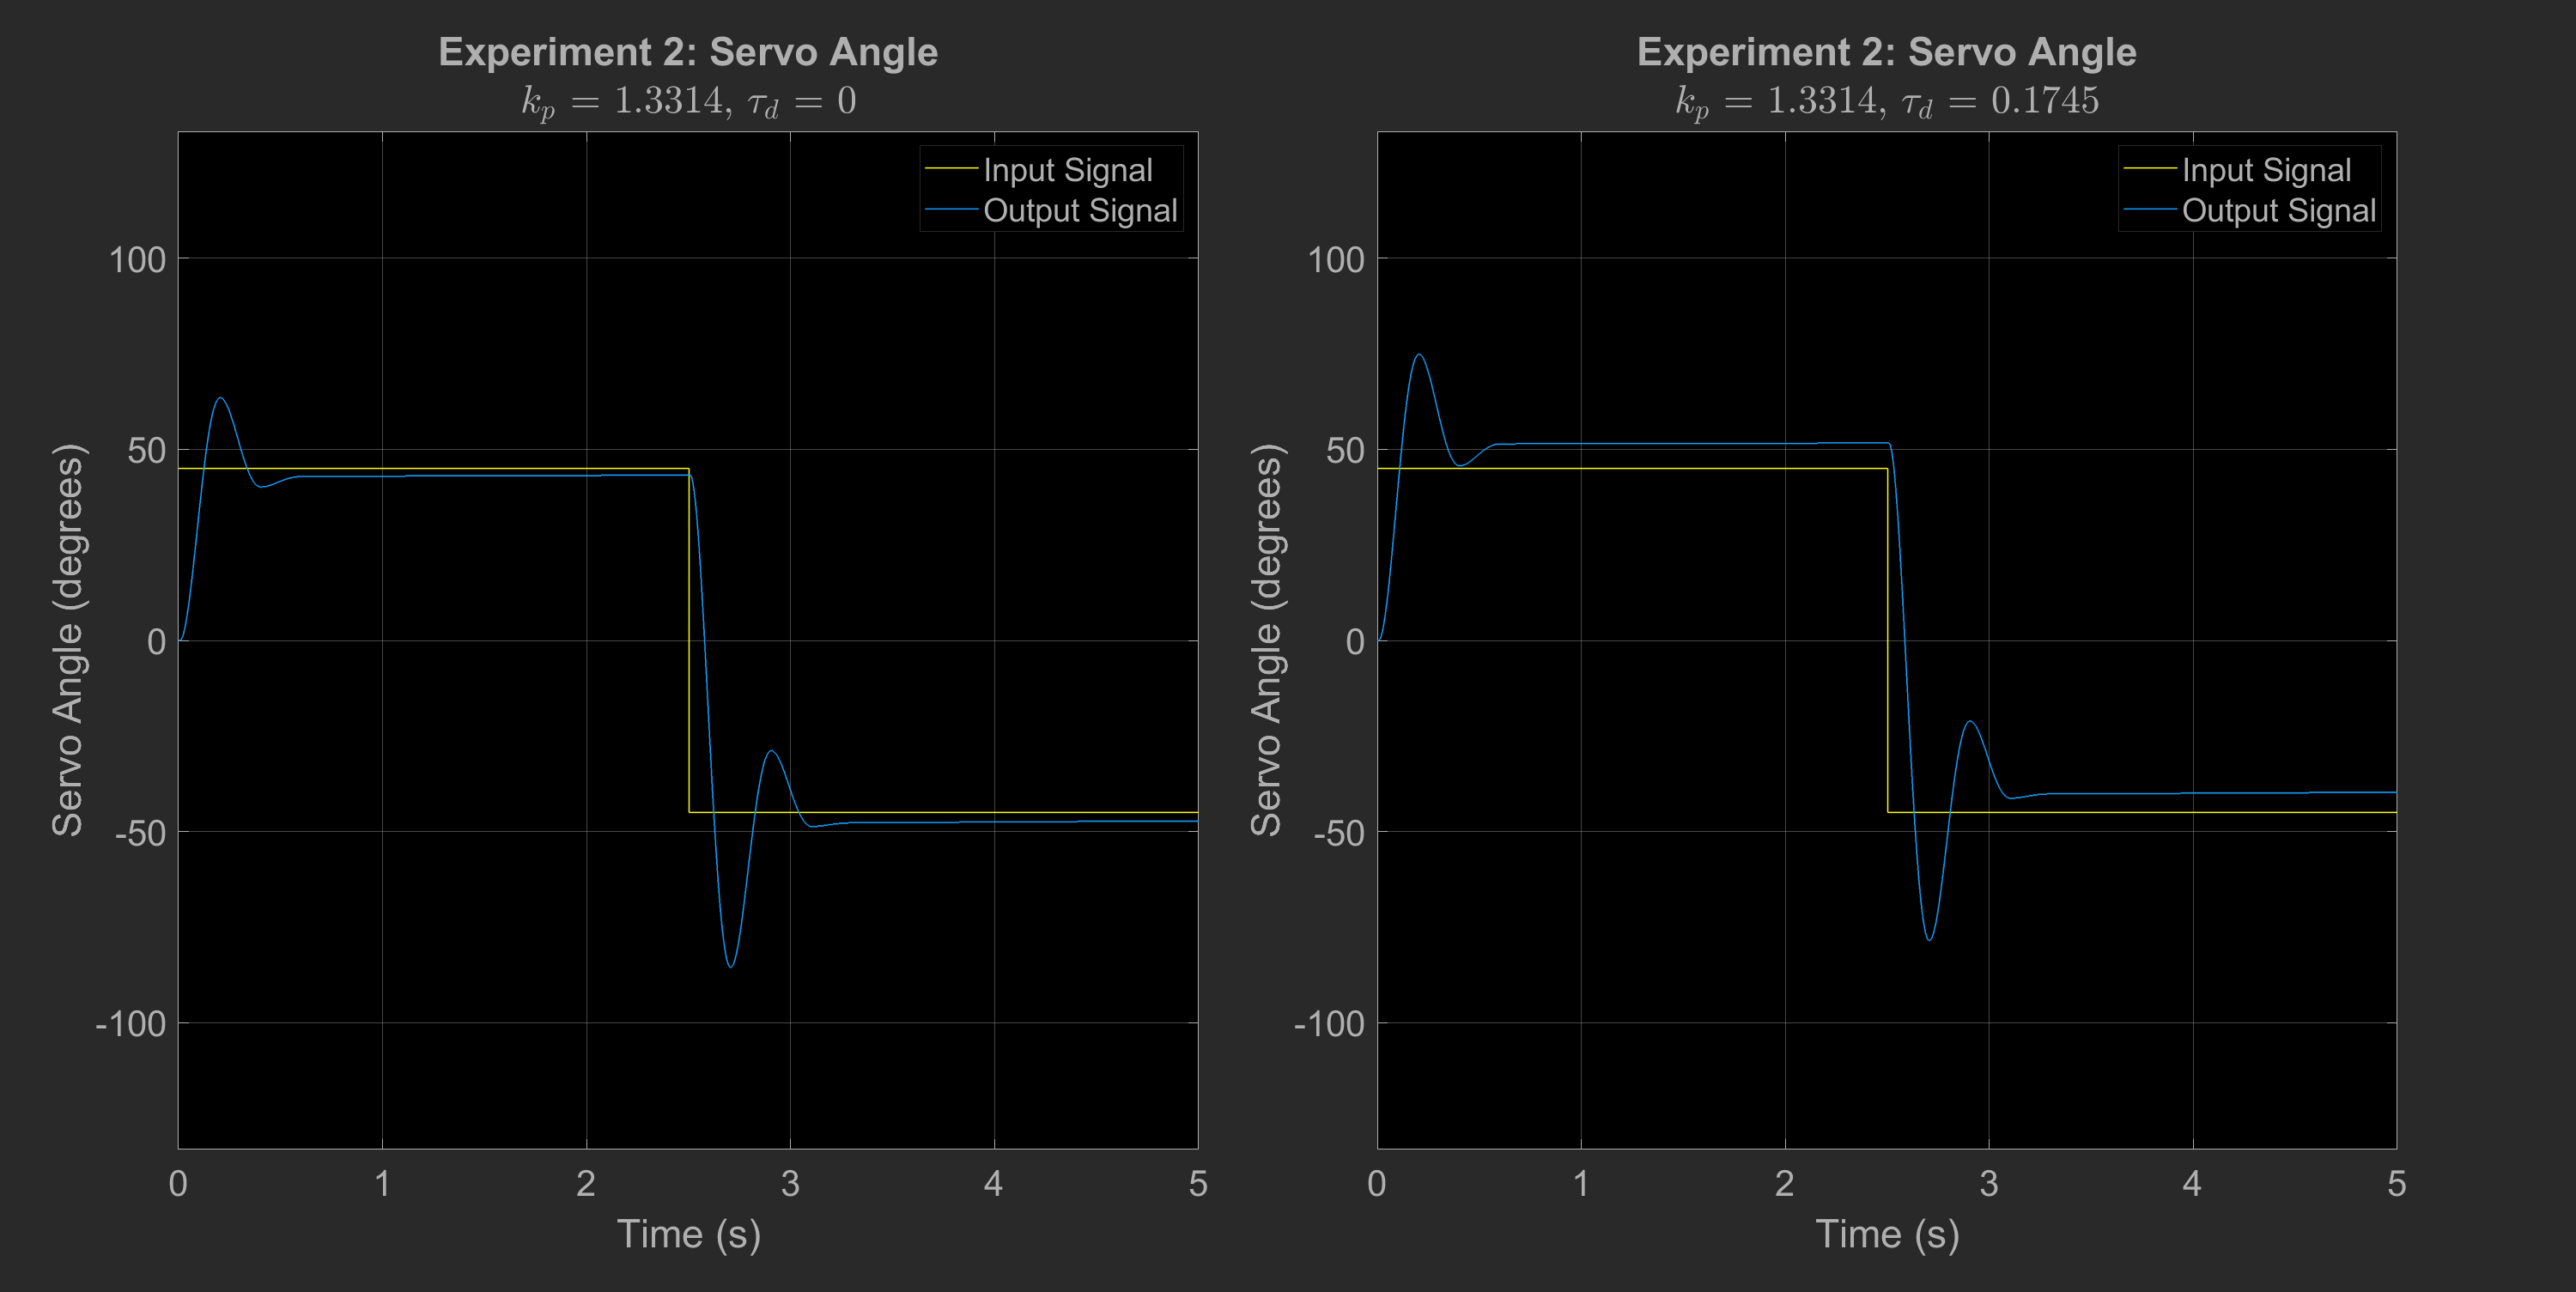
\includegraphics[width=0.91\textwidth]{exp2_kp1.3314}
    \caption{Experiment 2: $k_p = 1.3314$}
\end{figure}
\begin{figure}[h]
    \centering
    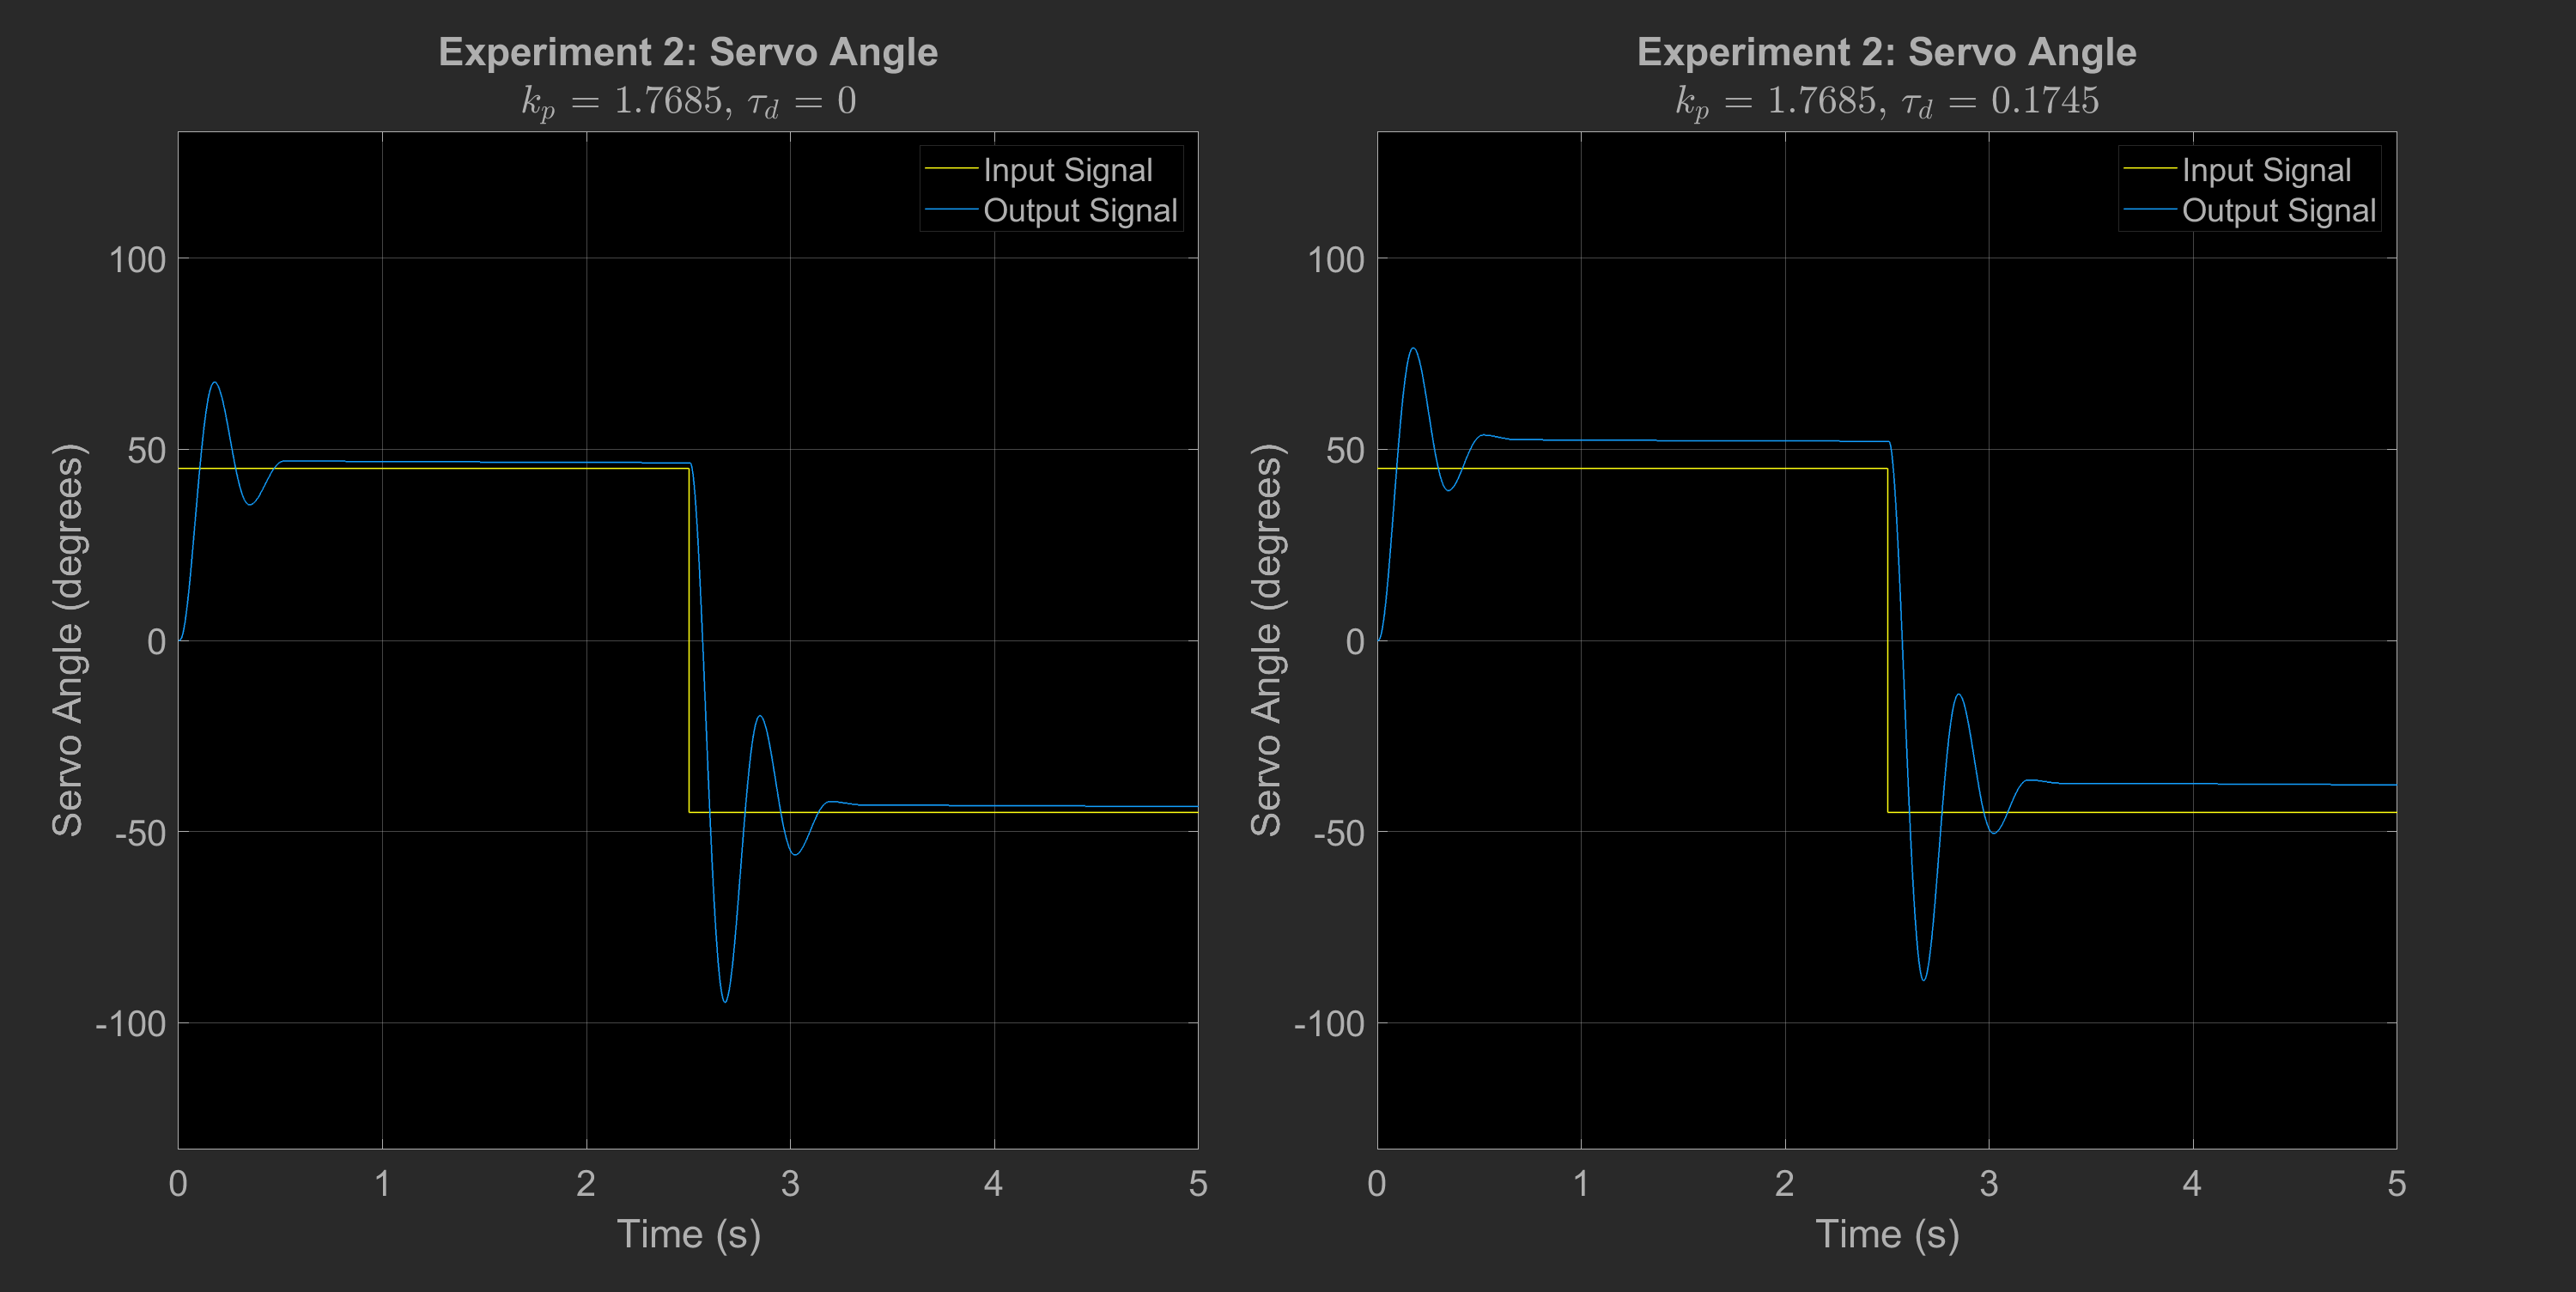
\includegraphics[width=0.91\textwidth]{exp2_kp1.7685}
    \caption{Experiment 2: $k_p = 1.7685$}
\end{figure}
\begin{figure}[h]
    \centering
    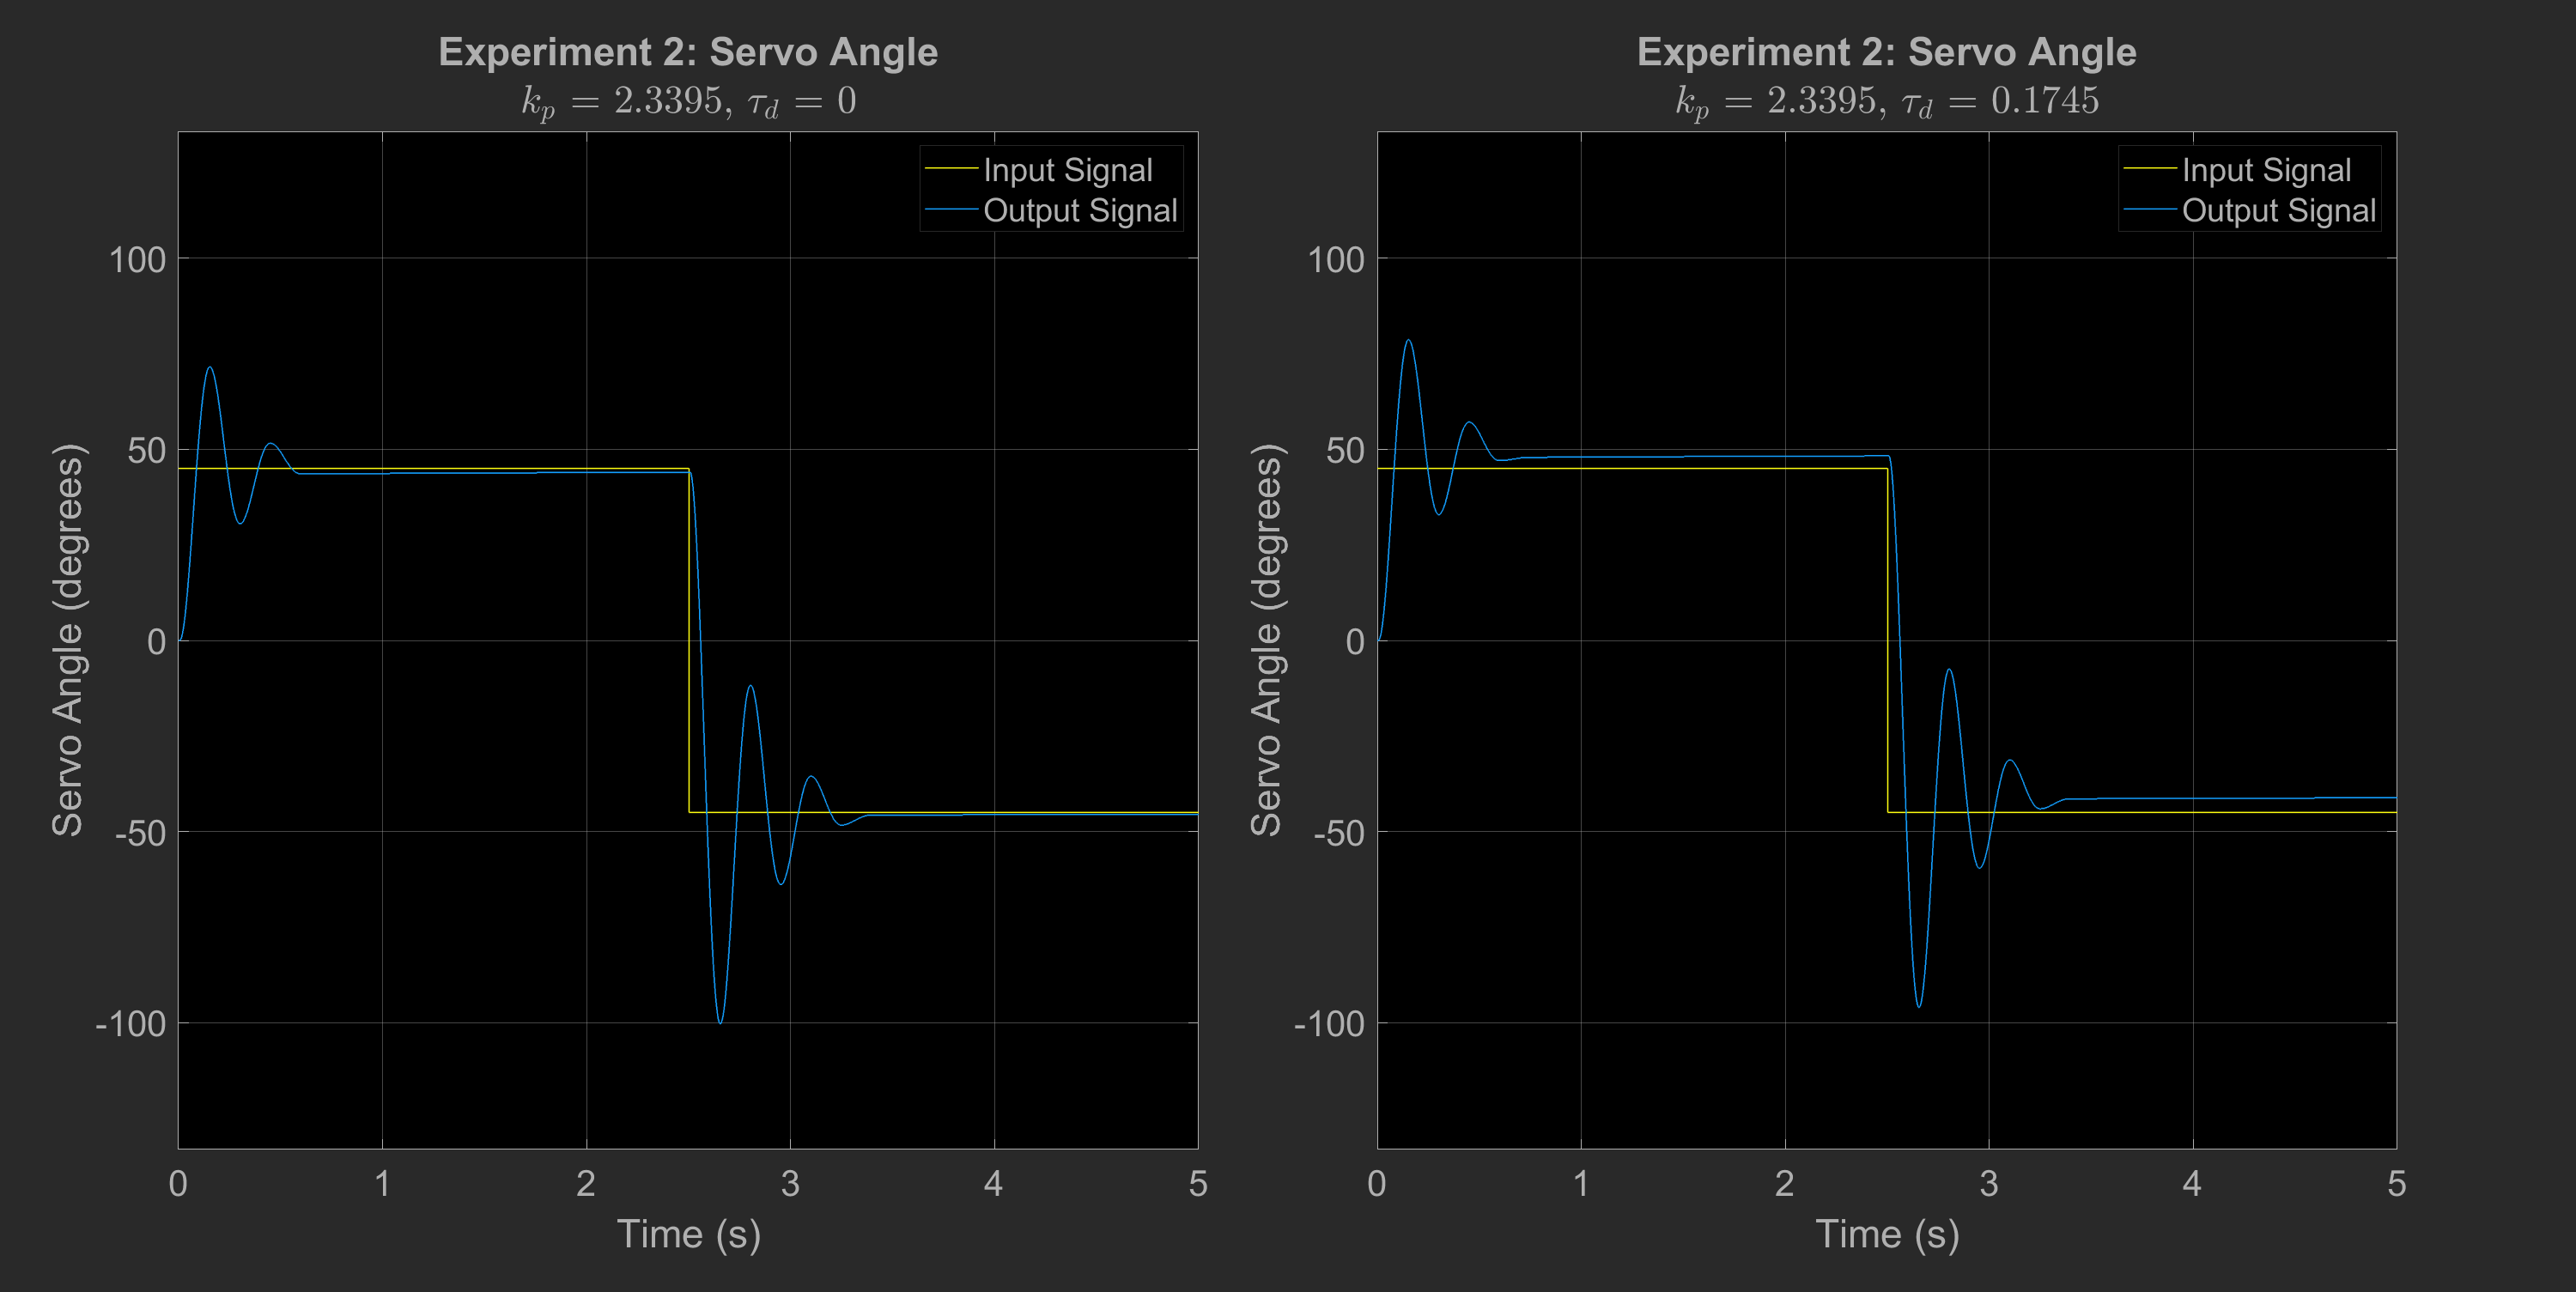
\includegraphics[width=0.91\textwidth]{exp2_kp2.3395}
    \caption{Experiment 2: $k_p = 2.3395$}
\end{figure}
\begin{figure}[h]
    \centering
    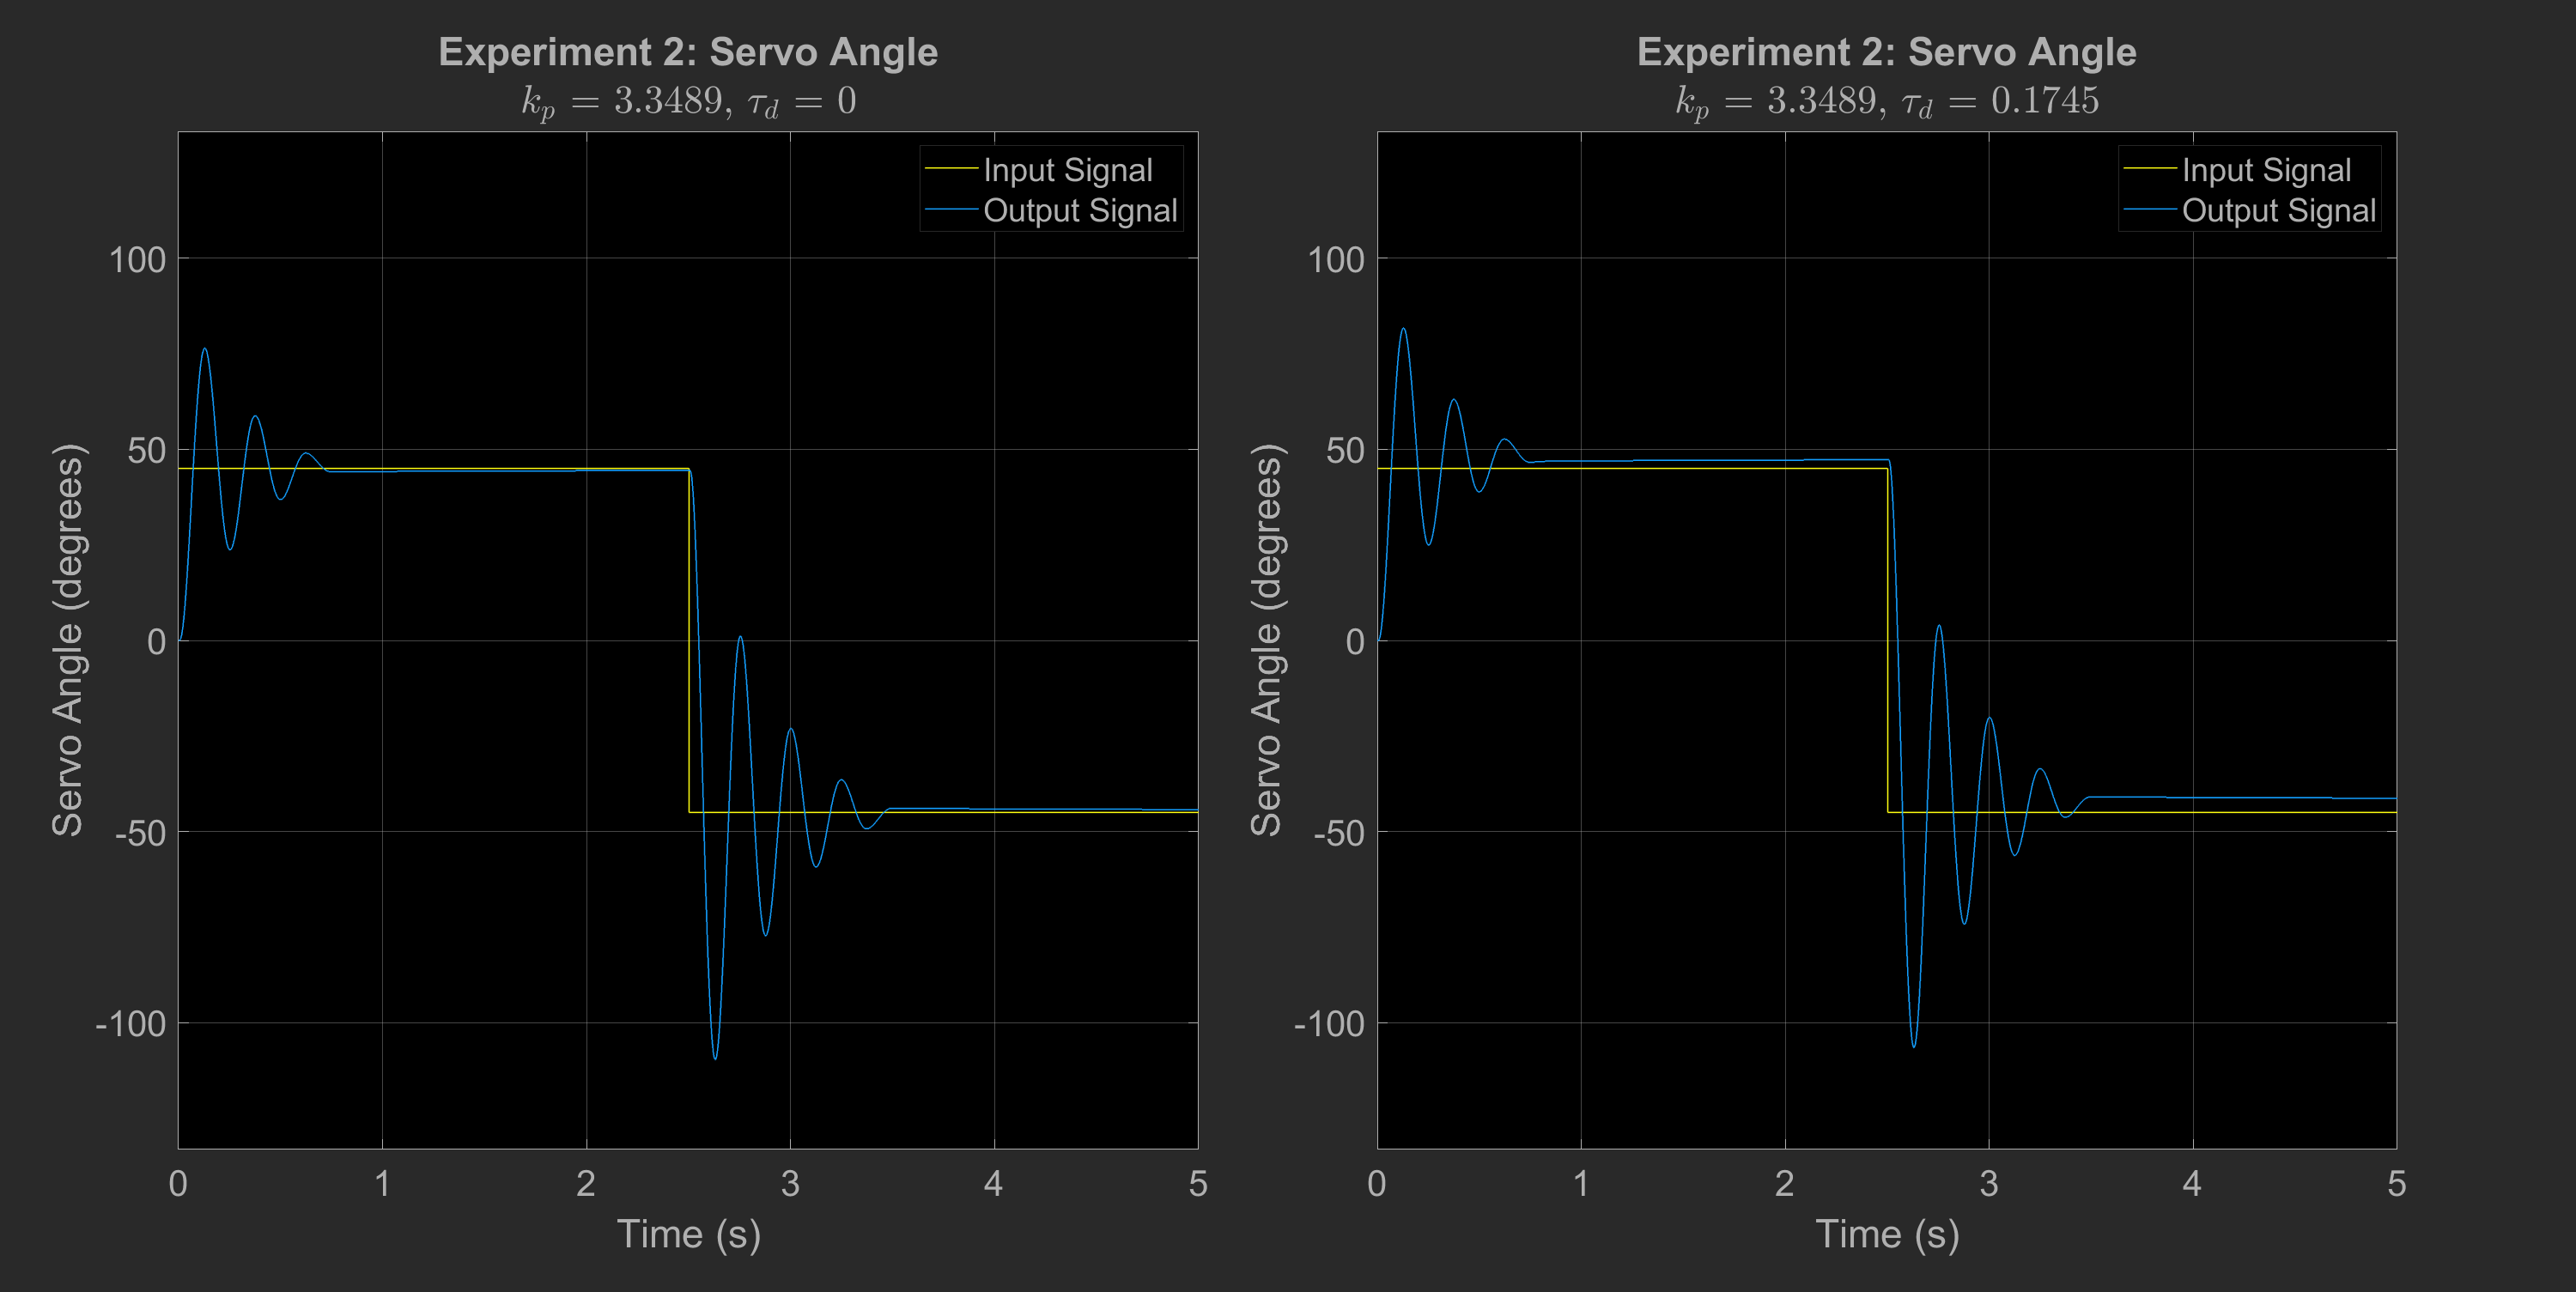
\includegraphics[width=0.91\textwidth]{exp2_kp3.3489}
    \caption{Experiment 2: $k_p = 3.3489$}
\end{figure}
\end{document}
